\documentclass[11pt,a4paper]{article}
\usepackage[T1]{fontenc}
\usepackage{lmodern}
\usepackage[margin=25mm,headheight=14pt]{geometry}
\usepackage{amsmath,amssymb,amsthm,mathtools}
\usepackage{booktabs,longtable,tabularx,array}
\usepackage{xcolor,microtype,listings}
\usepackage{fancyhdr,caption}
\usepackage{pgfplots}
\pgfplotsset{compat=1.18}
\usepackage{hyperref}
\hypersetup{colorlinks=true,linkcolor=blue!45!black,
 citecolor=blue!45!black,urlcolor=blue!45!black,
 pdftitle={Certified Prime Lifting and Sparse Modular Squaring},
 pdfauthor={KEIO},pdfsubject={Explicit certificates and exact-checked giant-integer arithmetic}}
\urlstyle{tt}
\definecolor{ink}{HTML}{18364B}
\definecolor{teal}{HTML}{007C83}
\definecolor{warm}{HTML}{C46A29}
\definecolor{codebg}{HTML}{F7F8FA}
\newtheorem{theorem}{Theorem}[section]
\newtheorem{proposition}[theorem]{Proposition}
\newtheorem{lemma}[theorem]{Lemma}
\newtheorem{corollary}[theorem]{Corollary}
\theoremstyle{definition}
\newtheorem{definition}[theorem]{Definition}
\newtheorem{remark}[theorem]{Remark}
\newcommand{\Z}{\mathbb Z}
\newcommand{\N}{\mathbb N}
\newcommand{\ord}{\operatorname{ord}}
\newcommand{\bits}{\operatorname{bits}}
\newcommand{\filecode}[1]{\texttt{\detokenize{#1}}}
\setlength{\emergencystretch}{2em}
\setlength{\parskip}{2.5pt}
\setlength{\parindent}{1.3em}
\setcounter{tocdepth}{1}
\captionsetup{font=small,labelfont=bf}
\pagestyle{fancy}
\fancyhf{}
\fancyhead[L]{\small\sffamily Certified Prime Lifting and Sparse Modular Squaring}
\fancyhead[R]{\small\sffamily KEIO}
\fancyfoot[C]{\thepage}
\renewcommand{\headrulewidth}{0.3pt}
\lstset{basicstyle=\ttfamily\fontsize{7.8}{9.4}\selectfont,
 numbers=left,numberstyle=\tiny\color{black!45},numbersep=6pt,
 keywordstyle=\color{ink}\bfseries,commentstyle=\color{black!57},
 stringstyle=\color{teal!85!black},backgroundcolor=\color{codebg},
 frame=single,rulecolor=\color{black!12},framesep=5pt,
 breaklines=true,breakatwhitespace=false,breakindent=12pt,
 showstringspaces=false,keepspaces=true,columns=fullflexible,
 tabsize=4,captionpos=t,xleftmargin=12pt,xrightmargin=3pt,
 aboveskip=12pt,belowskip=12pt}
\title{\color{ink}\bfseries Certified Prime Lifting\\and Sparse Modular Squaring\\[7pt]
 \large\normalfont An explicit prime certificate and arithmetic experiments\\at giant integer sizes}
\author{KEIO\\[3pt]\small Research development and manuscript preparation with ChatGPT}
\date{6 November 2026}
\begin{document}
\maketitle
\begin{abstract}
We document a completed prime-certification chain and a separate series of
arithmetic experiments on much larger unresolved candidates. Starting with
$14^{512}-14^{256}+1$, recursive Pocklington certificates establish seven
primes, culminating in an explicitly specified $18\,886$-digit integer.
For the externally certified Mersenne prime $q=2^{136279841}-1$, elementary
specializations of classical $N-1$ criteria show that each of $28q^2+1$ and
$66q^3+1$ would be certified by a completed base-two Fermat congruence;
neither congruence is evaluated here. We derive inversion-free execution
identities and prove three-fold quadratic and four-fold cubic reduction
bounds. At the full $82\,048\,642$-digit quadratic modulus, an existing FFT
engine is combined with exact signed conversion, direct limb assembly, and
first-fold fusion. Six rotating-order comparisons give a median of
$0.182662239$ seconds per checked modular square, $6.55\%$ below the
same-run direct-assembly baseline. All $18$ final results match complete
GMP reference integers. The resulting $1.58$-year multiplication of kernel
time by recurrence length is an extrapolation, not a completed primality
test or a production forecast. Proofs, counterexamples, certificates,
measurement data, and the frozen benchmark sources are included. No
historical-first or asymptotic-algorithm novelty is claimed.
\end{abstract}
\noindent\textbf{Keywords:} Pocklington certificate; prime lifting; sparse modular
reduction; FFT arithmetic; reproducible computation.
\clearpage
\tableofcontents
\clearpage
\section{Scope, contributions, and status}
\label{sec:scope}

An already certified prime supplies useful factorization information for a
larger candidate. It does not supply that candidate's primality automatically.
This distinction separates the two parts of this paper: a completed recursive
certificate for a specific integer, and arithmetic experiments on much larger
integers whose primality has not been decided.

The completed record is
\[
 r=62988p_5+1,
\]
where $p_5$ is defined by the explicit chain in Section~\ref{sec:record}.
The integer $r$ has $18\,886$ decimal digits and $62\,738$ bits. It is the
largest prime certified in the experimental record audited for this paper.
This statement is a project record, with no claim of a world record or a
historically first discovery of the integer.

The separate giant inputs are
\begin{equation}\label{eq:giants}
 p=136279841,\qquad q=2^p-1,\qquad
 N_2=28q^2+1,\qquad N_3=66q^3+1.
\end{equation}
The primality of $q$ is an established external result reported by GIMPS;
its original discovery and independent confirmations are described in the
2024 announcement~\cite{gimpsprime}. We use that result as an input and do
not rerun its Lucas--Lehmer test. Both $N_2$ and $N_3$ remain unresolved.
The main performance experiment concerns $x^2\bmod N_2$, at the actual
$272\,559\,687$-bit modulus size.

\begin{table}[htbp]
\centering\small
\caption{Objects and evidentiary status. A large input prime and a newly
certified project output are different roles.}
\label{tab:status}
\begin{tabularx}{\linewidth}{@{}l r X@{}}
\toprule
Object & Decimal digits & Status in this paper\\
\midrule
$p_0,\ldots,p_5$ & $587$--$18\,882$ & Complete recursive certificates verified.\\
$r=62988p_5+1$ & $18\,886$ & Complete Pocklington certificate verified.\\
$q=2^{136279841}-1$ & $41\,024\,320$ & Previously established external prime.\\
$N_2=28q^2+1$ & $82\,048\,642$ & Unresolved; bounded arithmetic experiments.\\
$N_3=66q^3+1$ & $123\,072\,962$ & Unresolved; derived arithmetic extension.\\
\bottomrule
\end{tabularx}
\end{table}

The substantive contributions of the record are an explicit, reproducible
certificate chain; fully stated specializations of classical order arguments;
constant-fold reduction bounds for the two sparse moduli; an exact treatment
of signed FFT conversion and the engine's internal modulus; and controlled
measurements with complete integer comparisons. The underlying Pocklington,
FFT, and special-modulus techniques are established. The paper makes no
claim of a new asymptotic multiplication algorithm or an unconditional formula
that always turns a prime into a larger prime.

All definitions, certificate parameters, reference algorithms, numerical
observations used in the principal comparison, and the complete measured
C++ benchmark source are contained in this document and its single LaTeX
source. Standard arithmetic libraries remain software dependencies.

\section{Classical certificates and prime lifting}
\label{sec:pocklington}

We use the following standard form of Pocklington's criterion
\cite{pocklington,bls}. A proof is included to make the certificate's logical
obligations explicit.

\begin{theorem}[Pocklington criterion]\label{thm:pocklington}
Let $n>1$ and let $F\mid n-1$ have known prime factorization, with
$F^2>n$. Then $n$ is prime if, for every distinct prime $\ell\mid F$,
there is an integer $a_\ell$ satisfying
\begin{equation}\label{eq:pockchecks}
 a_\ell^{n-1}\equiv1\pmod n,
 \qquad
 \gcd\bigl(a_\ell^{(n-1)/\ell}-1,n\bigr)=1.
\end{equation}
\end{theorem}

\begin{proof}
Let $s$ be any prime divisor of $n$. The first congruence makes $a_\ell$
a unit modulo $s$, with order dividing $n-1$. The gcd condition says that
this order does not divide $(n-1)/\ell$. Its $\ell$-adic valuation therefore
equals that of $n-1$, and in particular it contains the full $\ell$-power
occurring in $F$. Since the order divides $s-1$, we obtain $F\mid s-1$.
Thus every prime divisor $s$ of $n$ exceeds $F>\sqrt n$. A composite $n$
would have a prime divisor at most $\sqrt n$, a contradiction.
\end{proof}

No assumption $\gcd(F,(n-1)/F)=1$ is needed in this formulation. It happens
to hold in all seven certificates below. Different prime divisors of $F$
may use different witnesses.

\begin{corollary}[Reusable prime-power factor]\label{cor:lift}
Let $q$ be certified prime, $e\ge1$, and $1\le k<q^e$. Put
$n=kq^e+1$. If
\[
 a^{n-1}\equiv1\pmod n,
 \qquad \gcd\bigl(a^{kq^{e-1}}-1,n\bigr)=1,
\]
then $n$ is prime.
\end{corollary}

\begin{proof}
Use $F=q^e$. Since $k\le q^e-1$ and $q^e\ge2$,
$n\le q^{2e}-q^e+1<q^{2e}=F^2$.
\end{proof}

For an odd parent $q$, choosing even $k$ makes $n$ odd. One may sieve
candidates before evaluating the displayed congruences. A successful
certificate is reusable as the next parent. A failed Fermat congruence
proves compositeness; a failed gcd condition can instead mean that the
chosen base is unsuitable. For example, the prime parent $7$ with $e=2,k=2$ produces
$99$, which is composite. The construction is not a primality guarantee.

\subsection{Relation to other familiar methods}

\begin{table}[htbp]
\centering\small
\caption{Roles of classical methods. No performance comparison between these
different families is claimed here.}
\label{tab:methods}
\begin{tabularx}{\linewidth}{@{}l X X@{}}
\toprule
Method & Structure used & Role in the present work\\
\midrule
Pocklington & A sufficiently large factored portion of $n-1$. & Certifies the entire explicit chain.\\
Proth & $n=m2^t+1$, $m$ odd and $m<2^t$; an appropriate half-exponent witness. & Context for special-form certification.\\
Lucas--Lehmer & A dedicated recurrence for Mersenne numbers with prime exponent. & External certification context for the parent $q$.\\
ECPP & Elliptic-curve group-order and point certificates. & An alternative for less structured inputs; not used in the measurements.\\
\bottomrule
\end{tabularx}
\end{table}

Proth's criterion is a special $n-1$ method; classical extensions are discussed
by Brillhart, Lehmer, and Selfridge~\cite{bls}. The Lucas--Lehmer recurrence
is described in the GIMPS mathematical documentation~\cite{gimpsmath}.
ECPP uses a different certificate
structure, as developed by Atkin and Morain~\cite{atkinmorain}. Reusing a
large known factor of $n-1$ is attractive here because its factorization is
already built into the candidate. This observation does not establish
superiority over ECPP on general integers or over a tuned Lucas--Lehmer
implementation on Mersenne numbers.

\section{The explicit 18,886-digit certified record}
\label{sec:record}

Define
\begin{align}
 p_0&=14^{512}-14^{256}+1,\label{eq:seed}\\
 p_i&=k_i p_{i-1}^2+1\quad(1\le i\le5),\label{eq:chain}\\
 (k_1,k_2,k_3,k_4,k_5)&=(438,13696,5494,13258,22330),\notag\\
 r&=62988p_5+1.\label{eq:record}
\end{align}
These formulas specify each integer exactly without printing thousands of
decimal digits. The seed has the cyclotomic form $\Phi_6(14^{256})$.

\begin{table}[htbp]
\centering\small
\caption{The full certificate chain. Each row satisfies $F\mid n-1$ and
$F^2>n$. All listed witnesses passed both conditions in
\eqref{eq:pockchecks}.}
\label{tab:chain}
\begin{tabular}{@{}l r r l l@{}}
\toprule
Integer & Digits & Bits & Factored part $F$ & Witnesses $\ell:a_\ell$\\
\midrule
$p_0$ & 587 & 1,950 & $2^{256}7^{256}$ & $2:11$, $7:2$\\
$p_1$ & 1,177 & 3,908 & $p_0^2$ & $p_0:2$\\
$p_2$ & 2,357 & 7,829 & $p_1^2$ & $p_1:2$\\
$p_3$ & 4,718 & 15,670 & $p_2^2$ & $p_2:2$\\
$p_4$ & 9,439 & 31,354 & $p_3^2$ & $p_3:2$\\
$p_5$ & 18,882 & 62,722 & $p_4^2$ & $p_4:2$\\
$r$ & 18,886 & 62,738 & $p_5$ & $p_5:2$\\
\bottomrule
\end{tabular}
\end{table}

\begin{proposition}[Recorded computational certificate]\label{prop:record}
All seven integers in Table~\ref{tab:chain} are prime. The largest is $r$.
\end{proposition}

\begin{proof}[Certificate and verification]
Put $x=14^{256}$. For $p_0=x^2-x+1$, the known factor is
$F=x=2^{256}7^{256}$ and $F^2-p_0=x-1>0$. The two bases are $11$ for
$\ell=2$ and $2$ for $\ell=7$. At every quadratic step the certified factor
is $F=p_{i-1}^2$ and the base is $2$. At the final step $F=p_5$ and the
base is again $2$. The verifier in Appendix~\ref{app:certificate} reconstructs
the entire chain, checks divisibility and $F^2>n$, and evaluates all eight
witness pairs in \eqref{eq:pockchecks}. Each full power has residue $1$ and
each reduced-power gcd is $1$. Induction from the elementary primes $2$
and $7$, using Theorem~\ref{thm:pocklington}, proves the claim.
\end{proof}

For clarity, the final two computational obligations are
\begin{equation}\label{eq:finalcert}
 2^{r-1}\equiv1\pmod r,
 \qquad \gcd(2^{62988}-1,r)=1.
\end{equation}
The small gcd exponent in \eqref{eq:finalcert} does not remove the large
first exponent. Both were actually evaluated. At a quadratic step the
ordinary Pocklington gcd exponent is $k_i p_{i-1}$, not merely $k_i$.
The weaker small-exponent criteria in the next section are separate
arguments and are not substituted silently into this certificate.

Two full verification runs were completed afresh while preparing this
paper. The existing C/GMP verifier took $42.717327$ seconds and checked the
stored decimal integer. A separately implemented, self-contained Python
verifier using \texttt{gmpy2} took $42.765296$ seconds. Both passed all seven
nodes. These implementations provide separate certificate logic but share
the GMP arithmetic backend. The Python listing also has a standard-library
fallback; its slower complete large-integer run was not repeated here.

The previous recorded integer $5936p_5+1$ has $18\,885$ digits. It is
different from both the $18\,882$-digit parent $p_5$ and the present
$18\,886$-digit record $r$. We report no historical novelty for these
integers. Appendix~\ref{app:certificate} gives an unambiguous decimal hash.

\section{Small-exponent gcd criteria for the giant candidates}
\label{sec:criteria}

The order-divisibility mechanism below belongs to classical $n-1$ theory;
Theorem~6 of Brillhart--Lehmer--Selfridge~\cite{bls} provides the relevant
historical framework. We give the elementary specializations and their
size hypotheses explicitly. Their purpose is to specify exactly what a
completed computation would establish.

\begin{lemma}[Order forcing]\label{lem:order}
Let $q$ be prime, $e\ge1$, $1\le k<q$, and $n=kq^e+1$. If
\begin{equation}\label{eq:weakchecks}
 a^{n-1}\equiv1\pmod n,
 \qquad \gcd(a^k-1,n)=1,
\end{equation}
then every positive divisor of $n$ is congruent to $1$ modulo $q$.
\end{lemma}

\begin{proof}
For a prime $s\mid n$, the order of $a$ modulo $s$ divides $kq^e$ and
does not divide $k$. Since $q\nmid k$, the order is divisible by $q$.
Consequently $s\equiv1\pmod q$. Products of these primes, with their
multiplicities, give the assertion for all divisors.
\end{proof}

\begin{proposition}[Quadratic coefficient bound]\label{prop:quadcriterion}
Let $q$ be prime and $1\le k<q$. For $n=kq^2+1$, conditions
\eqref{eq:weakchecks} imply that $n$ is prime.
\end{proposition}

\begin{proof}
If $n$ were composite, Lemma~\ref{lem:order} would give a proper
factorization $n=(Aq+1)(Bq+1)$ with integers $A,B\ge1$. Comparing
coefficients gives
\[
 q(k-AB)=A+B>0.
\]
Hence $AB\le k-1$, while
$A+B\le AB+1\le k<q$, contradicting the displayed positive multiple of $q$.
\end{proof}

\begin{proposition}[Cubic coefficient bound]\label{prop:cubiccriterion}
Let $k>1$ be an integer that is not a perfect cube. Let $q$ be prime with
$q>4k^2$, and put $n=kq^3+1$. Conditions \eqref{eq:weakchecks} imply that
$n$ is prime.
\end{proposition}

\begin{proof}
Here $k<q$, so a composite $n$ would have a factorization
$n=(Aq+1)(Bq+1)$, with $1\le A\le B$. There is an integer $t\ge1$ such that
\begin{equation}\label{eq:cubicfactors}
 A+B=tq,\qquad AB=kq-t.
\end{equation}
The inequality $A+B\le AB+1$ yields $t(q+1)\le kq+1$, so $t<k$ because
$k>1$. Also
\[
 \frac A2\le\frac{AB}{A+B}=\frac{kq-t}{tq}<\frac{k}{t}\le k,
\]
and therefore $A<2k$. Eliminating $B$ from \eqref{eq:cubicfactors} gives
\[
 q(At-k)=A^2-t.
\]
The right side has absolute value less than $4k^2<q$. Both sides must
vanish, giving $t=A^2$ and $k=A^3$, contrary to the hypothesis.
\end{proof}

\subsection{Exact specialization to base two}

For the exponent in \eqref{eq:giants}, direct integer remainders give
\[
 p\equiv5\pmod{28},\qquad p\equiv5\pmod{66}.
\]
Thus $q\equiv31\pmod{2^{28}-1}$ and $q\equiv31\pmod{2^{66}-1}$.
The two required small gcd values are
\begin{align}
 \gcd(N_2,2^{28}-1)
 &=\gcd(26909,268435455)=1,\label{eq:gcd28}\\
 \gcd(N_3,2^{66}-1)
 &=\gcd(1966207,73786976294838206463)=1.\label{eq:gcd66}
\end{align}
Since $28<q$, $66$ is not a cube, and $q>4\cdot66^2$, the preceding
propositions prove the following exact equivalences:
\begin{equation}\label{eq:fermatiff}
 \boxed{\quad
 N_j\text{ is prime}\quad\Longleftrightarrow\quad
 2^{N_j-1}\equiv1\pmod{N_j},\qquad j\in\{2,3\}.
 \quad}
\end{equation}
Necessity is Fermat's theorem; sufficiency uses the stated structure and
gcd computations. An arbitrary base-two Fermat pseudoprime is not covered
by \eqref{eq:fermatiff}.

Neither full congruence in \eqref{eq:fermatiff} has been computed for the
giant targets in this record. The small gcd calculations are inexpensive
preconditions; they do not decide primality by themselves. A completed
residue unequal to $1$ would establish compositeness, whereas an unfinished run
has no such implication.

\section{Inversion-free execution identities}
\label{sec:recurrence}

The quadratic Fermat congruence has a useful execution form requiring only
successive squaring and one final multiplication by a small power of two.

\begin{proposition}[Quadratic recurrence]\label{prop:recurrence}
Let $p\ge1$, $N=28(2^p-1)^2+1$, $u=2^{28}$, and
\[
 x_0=u\bmod N,\qquad x_{i+1}=x_i^2\bmod N.
\]
Then
\begin{equation}\label{eq:recurrencecheck}
 2^{N-1}\equiv1\pmod N
 \quad\Longleftrightarrow\quad
 u x_{2p}\equiv x_{p+1}\pmod N.
\end{equation}
\end{proposition}

\begin{proof}
We have $x_i\equiv u^{2^i}\pmod N$. Since $N$ is odd, $u$ is a unit.
The difference of the exponents on the right of
\eqref{eq:recurrencecheck} is
\[
 1+2^{2p}-2^{p+1}=(2^p-1)^2.
\]
Cancellation of a unit is legitimate in the proof; the implementation
needs no modular inversion.
\end{proof}

An execution stores $C=x_{p+1}$, continues to $X=x_{2p}$, and compares
$uX\bmod N$ with $C$. For the actual target this uses exactly
\begin{equation}\label{eq:squarecount}
 2p=272\,559\,682
\end{equation}
modular squarings, plus the final shift-and-reduce operation. This is a
count for this recurrence, not a lower bound for every possible algorithm.
Successive states depend on preceding states; parallelizing one large
square does not make the recurrence's time steps independent.

For completeness, the cubic identity is also inversion-free. With
$N=66(2^p-1)^3+1$, $u=2^{66}$, and the same squaring recurrence,
\begin{equation}\label{eq:cubicrecurrence}
 2^{N-1}\equiv1\pmod N
 \Longleftrightarrow
 x_{3p}x_p^3\equiv u x_{2p}^3\pmod N.
\end{equation}
Indeed, the exponent difference is
$2^{3p}+3\cdot2^p-3\cdot2^{2p}-1=(2^p-1)^3$.
One can retain $x_p,x_{p+1},x_{2p},x_{2p+1}$ along the chain and form
$x_p^3=x_p x_{p+1}$ and $x_{2p}^3=x_{2p}x_{2p+1}$.
Thus the implementation uses $3p=408\,839\,523$ chain squarings, three
additional general modular multiplications, and a final multiplication by
$u$, implemented as a 66-bit shift and reduction. It is not a
$3p$-operation complete implementation. No giant cubic recurrence was run.

\section{Exact reduction for the sparse moduli}
\label{sec:reduction}

Reduction tailored to a special modulus is a classical technique
\cite{solinas,bajard}. Here all constants and stopping bounds are proved
for the particular quadratic and cubic expressions. The reduction identities
do not assume that the modulus or its Mersenne parent is prime.

\subsection{A three-fold quadratic reducer}

Let $p\ge8$, $B=2^p$, and
\begin{equation}\label{eq:Acquad}
 A=28B^2,\quad c=56B-29,\quad N=A-c.
\end{equation}
For $T\ge0$, define
\begin{equation}\label{eq:fold}
 \mathcal F(T)=(T\bmod A)+\lfloor T/A\rfloor c.
\end{equation}
Because $A\equiv c\pmod N$, this preserves the residue modulo $N$.
Write $T=HB^2+L$, with $0\le L<B^2$, and $H=28h+s$, with $0\le s<28$.
Then the exact implementable expression is
\begin{equation}\label{eq:foldimpl}
 \mathcal F(T)=L+sB^2+56hB-29h.
\end{equation}
Splitting at bit $2p$ uses shifts and masks. Division of $H$ by $28$ is
division of a large integer by a fixed small integer; its cost is linear
in the limb count, rather than constant time.

\begin{theorem}[Three folds suffice]\label{thm:threefold}
If $p\ge8$ and $0\le T<N^2$, then $T_3=\mathcal F^3(T)$ satisfies
$0\le T_3<2N$. Therefore three folds followed by at most one subtraction
of $N$ give $T\bmod N$.
\end{theorem}

\begin{proof}
Since $N<A$ and $T<A^2$, the first fold obeys $T_1<A(c+1)$.
The second quotient is at most $c$, so
\[
 T_2\le A-1+c^2<113A,
\]
where $c^2<112A$ follows immediately from $c<56B$.
Thus the third quotient is at most $112$, and
\[
 T_3\le A-1+112c.
\]
Finally,
\[
 A-114c+1=28B^2-6384B+3307>0\qquad(B\ge256).
\]
The polynomial is positive at $256$ and increasing thereafter. Hence
$A-1+112c<2(A-c)=2N$. Nonnegativity follows from $0<c<A$ and
\eqref{eq:fold}.
\end{proof}

\begin{corollary}[Small final quotient]\label{cor:smalllast}
Under the hypotheses of Theorem~\ref{thm:threefold}, the last quotient
$h=\lfloor T_2/A\rfloor$ is at most $112$. The last correction in
\eqref{eq:foldimpl} uses $56h\le6272$ and $29h\le3248$.
\end{corollary}

This bound permits a direct shifted-small-integer update instead of allocating
a long mostly-zero temporary. Carry propagation must still be correct for
arbitrarily long runs of zero or one limbs. The bound does not justify
assuming that a carry always stops after one machine word.

For fixed coefficient $28$, the reducer requires $O(L)$ limb work for an
$L$-bit modulus, in addition to the $M(L)$ cost of the square. Thus the
one-step cost has the form $M(L)+O(L)$ in the usual arithmetic model.
This is not an asymptotic improvement over all optimized modular
multiplication methods.

\subsection{A four-fold cubic extension}

For $p\ge13$ and $B=2^p$, put
\[
 A=66B^3,\qquad c=198B^2-198B+65,\qquad N=A-c.
\]
The fold \eqref{eq:fold} again preserves residues. Splitting at bit $3p$
and writing $H=66h+s$ gives
\[
 \mathcal F(T)=L+sB^3+198hB^2-198hB+65h.
\]

\begin{proposition}[Four cubic folds]\label{prop:fourfold}
For $p\ge13$ and $0\le T<N^2$, four folds followed by at most one
subtraction of $N$ give the canonical remainder.
\end{proposition}

\begin{proof}
As before, $T_1<A(c+1)$ and $T_2<A+c^2$. Consequently
$T_3<A+c+c^3/A$. Since $c<198B^2$,
\[
 \frac{T_3}{A}<1+\frac{3}{B}
    +\frac{198^3B^6}{66^2B^6}
   =1783+\frac3B<1784.
\]
The fourth quotient is at most $1783$, so
$T_4\le A-1+1783c$. For $B\ge8192$,
$A=66B^3>1785c$, using $1785\cdot198/66=5355<B$.
It follows that $T_4<2(A-c)=2N$.
\end{proof}

The cubic reducer is a derived extension with exact small-input controls.
It has not been benchmarked at the full $N_3$ size. A change of notation
alone does not improve the quadratic reducer: for odd $p$, writing
$R=2^{(p+1)/2}$ gives $N_2=7R^4-28R^2+29$, but its $A$ and $c$ are
exactly those in \eqref{eq:Acquad}.

\section{Exact conversion around the FFT engine}
\label{sec:fft}

FFT-based large-integer multiplication and weighted transforms are established
methods~\cite{crandallfagin}. The measured implementation uses the existing
GWnum engine and exact GMP integer operations~\cite{gimpssoftware,gmp}.
Its new code arranges conversions and reduction around that engine.

\subsection{Padding and the internal modulus}

The non-modular setup is requested with an output capacity of $2L+2$ bits,
where $L=\bits(N_2)$. The selected internal representation uses
\[
 M=2^n-1,\qquad n\ge2L+2.
\]
For $0\le x<N_2<2^L$, we have $x^2<2^{2L}<M$. Hence the canonical
engine residue modulo $M$ is the ordinary integer square. The actual setup
selected $n=545\,119\,376$ and an FFT length of $31\,457\,280$.

The distinction between $M$ and $N_2$ is essential. An unnormalized signed
FFT polynomial can equal $x^2+tM$ for nonzero $t$. Reducing that raw
polynomial directly modulo $N_2$ may be wrong, because $M$ is generally
nonzero modulo $N_2$. The internal normalization must be performed first,
even when its result is kept in split form.

\subsection{Parallel balanced import}

Let $0=e_0<e_1<\cdots<e_D=n$ be FFT bit boundaries, with
$b_i=2^{e_{i+1}-e_i}$. Let $r_i$ be the ordinary unsigned digits of $x$.
Set $c_0=0$ and, for $i>0$, let $c_i$ be the bit of $x$ at position
$e_i-1$. Define
\begin{equation}\label{eq:balancedimport}
 d_i=r_i+c_i-b_i c_{i+1}.
\end{equation}
The digits can be calculated independently. Multiplying by $2^{e_i}$ and
summing telescopes to
\[
 \sum_{i=0}^{D-1}d_i2^{e_i}=x-c_D2^n.
\]
The padding ensures $x<2^{n-1}$, hence $c_D=0$ and the sum equals $x$.
The inclusive bounds $-b_i/2\le d_i\le b_i/2$ allow a positive half-radix
tie. The weaker condition $x<2^n$ alone would not force the required
zero top carry.

\subsection{Direct signed-chunk export}

For a chunk of width $W_j$, pack its signed polynomial by exact Euclidean
division into
\[
 S_j=R_j+q_j2^{W_j},\qquad 0\le R_j<2^{W_j}.
\]
With incoming carry $C_0=0$, normalize consecutive chunks by
\begin{align}
 R'_j&=(R_j+C_j)\bmod2^{W_j},\label{eq:stitch}\\
 C_{j+1}&=q_j+\left\lfloor\frac{R_j+C_j}{2^{W_j}}\right\rfloor.\notag
\end{align}
This gives the exact total representation
\begin{equation}\label{eq:globalcarry}
S=U+C_{\mathrm{top}}2^n,\qquad 0\le U<2^n,
\end{equation}
where $C_{\mathrm{top}}$ is the carry above the last export chunk.
Therefore the engine residue is $(U+C_{\mathrm{top}})\bmod M$.

The implementation supports arbitrary rounded signed 32-bit coefficients.
An elementary digit-by-digit carry recurrence preserves the signed 32-bit
carry range, since every radix is at least two. With $n\ge33$, the value
$U+C_{\mathrm{top}}$ lies strictly between $-M$ and $2M$, so at most one correction by
$M$ is needed. No assumption of nonnegative chunks is made.

Implemented chunks satisfy $W_j\ge32$, so a signed 32-bit incoming carry
has magnitude below the chunk radix. Internal chunk boundaries are aligned
with 64-bit limbs. Workers write
disjoint output regions; the short chain of boundary carry corrections is
performed afterwards. A final partial limb is masked at its actual bit
boundary. Positive overflow above that boundary, rather than merely overflow
above the machine word, supplies its outgoing carry. Negative updates retain
the true borrow before masking. GMP's low-level operations permit these
subrange and in-place updates under their documented size and overlap
conditions~\cite{gmp}.

\subsection{Split normalization and fusion}

The combined exporter keeps low and high buffers around a chosen split
$s=2p$. Write $D_0=2^s$, $E=2^{n-s}$, and $M=D_0E-1$. After the lower
piece is floor-normalized, write the exact signed polynomial as
$S=H_0D_0+L_0$, where $0\le L_0<D_0$. Decompose $H_0=QE+H_1$, with
$0\le H_1<E$, and transfer the quotient $Q$ into the low piece. After
normalizing that piece again, the resulting pair $(H,L)$ represents
\[
 V=HD_0+L=(S\bmod2^n)+\lfloor S/2^n\rfloor.
\]
We have $-M<V<2M$ and $V\equiv S\pmod M$. The final correction can be
done without constructing a complete product:
\begin{itemize}
\item If $H<0$, add $E$ to the high part and subtract one from the low
part, normalizing its carry. This adds $M$.
\item If $H\ge E$, subtract $E$ and add one to the low part. This
subtracts $M$.
\item If $H=E-1$ and $L=D_0-1$, replace both parts by zero.
\end{itemize}
Thus the pair is the exact canonical engine residue. The code implements
the additions or subtractions of powers of two through masks and bounded
carries. It then applies \eqref{eq:foldimpl} directly to the two buffers,
followed by the two remaining target-modulus folds.

An FFT-word boundary need not coincide with bit $2p$. The selected boundary
in the giant experiment is $272\,559\,671$, eleven bits below $2p$.
The code transfers that gap exactly and aligns chunks relative to each
buffer's own origin. The complete source in Appendix~\ref{app:cpp} retains
guards for unsupported layouts, finite conversion values, signed carry
range, and FFT error checks.
\section{Implementation and experimental design}
\label{sec:experiments}

\subsection{Measured arithmetic and hardware}

All principal timings use the actual modulus $N_2$ in \eqref{eq:giants}.
The host reports an AMD EPYC 9V74 processor with AVX-512. The container
has a quota of eight CPU cores, affinity to logical indices $0$ through
$8$, and an $8$~GiB memory limit. The kernels use eight threads. The
recorded compiler is GCC $13.3.0$, the exact-integer library is GMP
$6.3.0$, and the FFT engine is GWnum $31.6$. Source versions, compilation
arguments, and fingerprints are specified in Appendix~\ref{app:cpp}.

The candidate implementations use the same deterministic initial dense
residue. Each subsequent input is the preceding exact square modulo $N_2$.
The six final inputs are successive arithmetic states, not six independent
random observations and not the initial states of the full Fermat recurrence.
Structured small inputs were tested separately.

For each input, a reference GMP square and general remainder are computed
before timing any candidate variant. The timed interval is uninterrupted:
input conversion, FFT squaring, output conversion including any fused first
fold, remaining sparse folds, and roundoff/error checks. Whole-integer
comparison with the reference occurs after the timer. In the direct-export
experiments, the unchanged FFT output is also re-exported after the timer
to compare the entire raw square with GMP.

Setup, upfront allocation, reference arithmetic, post-timer comparisons,
logging, and prospective long-run fault-management costs are excluded.
Allocations or thread-management operations performed inside the timed
code are included. The prototype therefore measures an arithmetic kernel,
not the wall time of a fault-tolerant complete primality test.

\subsection{Controlled comparisons, including non-improvements}

\begin{table}[htbp]
\centering\small
\caption{Four bounded comparisons at the full quadratic modulus. Values are
medians of complete timed kernels in seconds. Each experiment is a separate
execution; comparisons across experiments are observational.}
\label{tab:ablations}
\begin{tabularx}{\linewidth}{@{}l X r@{}}
\toprule
Experiment & Variant & Median (s)\\
\midrule
A: five pairs & Horner assembly, three folds & 0.234083010\\
 & Direct limb assembly, three folds & 0.192841305\\
\addlinespace
B: five pairs & Horner assembly, three folds & 0.214489496\\
 & Two-piece Horner fusion, two remaining folds & 0.210054299\\
\addlinespace
C: five pairs & Direct assembly, ordinary last fold & 0.187881590\\
 & Direct assembly, scalar last fold & 0.192677406\\
\addlinespace
D: six triples & Direct assembly, three folds & 0.195463347\\
 & Direct split fusion, ordinary last fold & 0.188044851\\
 & Direct split fusion, scalar last fold & \textbf{0.182662239}\\
\bottomrule
\end{tabularx}
\end{table}

Experiment A isolates the effect of replacing growing Horner assembly by
direct limb writes. It reduced median complete-kernel time by $17.62\%$;
the median export phase fell from $0.097076133$ to $0.065709379$ seconds.
All ten complete raw squares and all ten remainders matched the references.

Experiment B shows that splitting the product while retaining Horner
assembly has only a small observed median benefit. Experiment C does not
show an end-to-end improvement from the scalar last fold alone. These runs
are retained, including their scheduling outliers; no samples were discarded.
A mathematical simplification is not automatically a measured speedup.

Experiment D combines direct assembly with split normalization and first-fold
fusion. Its order rotates among the three methods. Each method occupies
each execution position exactly twice. The scalar-last-fold combination has
the lowest median, $0.182662239$ seconds, and is faster than the direct
baseline on all six inputs. Relative to that baseline, the median time is
$6.55\%$ lower, a speed ratio of $1.0701$. Relative to fusion with the
ordinary last fold, its median is about $2.86\%$ lower. Six bounded
observations do not establish a universal performance advantage.

\begin{figure}[htbp]
\centering
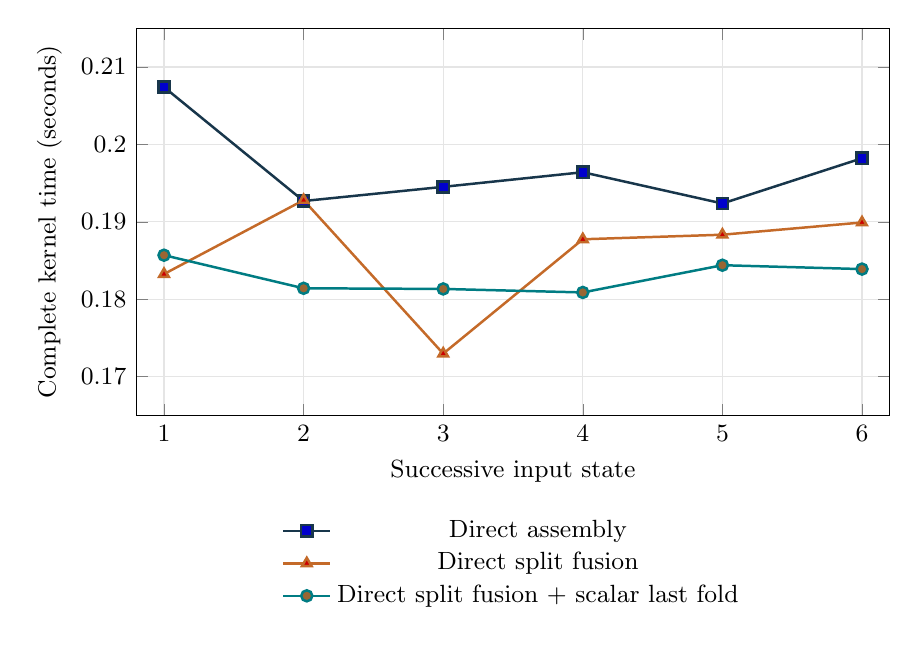
\begin{tikzpicture}
\begin{axis}[
 width=0.92\linewidth,height=6.5cm,
 xlabel={Successive input state},ylabel={Complete kernel time (seconds)},
 xmin=0.8,xmax=6.2,xtick={1,2,3,4,5,6},ymin=0.165,ymax=0.215,
 ytick={0.17,0.18,0.19,0.20,0.21},
 scaled y ticks=false,yticklabel style={/pgf/number format/fixed,
 /pgf/number format/precision=2},grid=major,grid style={black!10},
 tick label style={font=\small},label style={font=\small},
 legend style={at={(0.5,-0.24)},anchor=north,draw=none,
 font=\small,legend columns=1},
 ]
\addplot+[color=ink,mark=square*,line width=0.9pt] coordinates {(1,0.207395623) (2,0.192690529) (3,0.194519957) (4,0.196406737) (5,0.192371685) (6,0.198213349)};
\addlegendentry{Direct assembly}
\addplot+[color=warm,mark=triangle*,line width=0.9pt] coordinates {(1,0.183262043) (2,0.192801010) (3,0.172984908) (4,0.187750568) (5,0.188339135) (6,0.189920092)};
\addlegendentry{Direct split fusion}
\addplot+[color=teal,mark=*,line width=0.9pt] coordinates {(1,0.185696162) (2,0.181422296) (3,0.181339547) (4,0.180888095) (5,0.184402325) (6,0.183902183)};
\addlegendentry{Direct split fusion + scalar last fold}
\end{axis}
\end{tikzpicture}
\caption{All six observations in the final rotating-order comparison.
Lines identify methods across successive states; they do not represent
independent replications or a fitted trend.}
\label{fig:paired}
\end{figure}


All $18$ remainders in experiment D match the full GMP reference integers.
The winning variant's sample times range from $0.180888095$ to
$0.185696162$ seconds. The entire final benchmark process, including
setup and reference arithmetic, ran for $42.641879$ seconds and reached
$1\,052\,040$~KiB peak child-process RSS. That memory figure describes
the benchmark process and is not a separately measured production footprint.
The four comparisons together contain $48$ checked implementation-run
remainders on a reused input sequence. Their exact sample data appear in
Appendix~\ref{app:measurements}.

\subsection{Earlier stages and time scaling}

The work progressed from a generic remainder operation to a sparse reducer,
then to lower-overhead integer code and an FFT-based square. Table~\ref{tab:history}
records selected milestones. These stages differ in implementation and, in
some cases, thread count and timing harness. They must not be combined into
a single controlled treatment estimate.

\begin{table}[htbp]
\centering\small
\caption{Selected earlier and final observations. The last column merely
multiplies the kernel median by $272\,559\,682$ and divides by
$365.25\cdot86400$; it is not a completion forecast.}
\label{tab:history}
\begin{tabularx}{\linewidth}{@{}X r r@{}}
\toprule
Recorded implementation & Seconds/step & Scaled years\\
\midrule
Initial generic GMP square and remainder & 8.060205099 & 69.62\\
Sparse reducer through Python/GMP & 1.692279614 & 14.62\\
C++ sparse reducer with reused buffers & 1.376366940 & 11.89\\
Seven parallel sub-squares with GMP & 0.682184970 & 5.89\\
GWnum with stock conversions & 0.686471842 & 5.93\\
GWnum with parallel input/output conversion & 0.235293538 & 2.03\\
Final direct split fusion with scalar last fold & 0.182662239 & 1.58\\
\bottomrule
\end{tabularx}
\end{table}

The first sparse-reduction comparison also included a contemporaneous generic
GMP median of $7.090269219$ seconds, yielding a within-run ratio of $4.1898$
against $1.692279614$ seconds. The historical $8.060205099$-second figure
belongs to another run. In the preceding parallel-conversion revision, the
reported total summed measured segments separated by reference work; the
current paired and triple harnesses time a contiguous kernel. This is an
additional reason to emphasize the within-run comparisons in
Table~\ref{tab:ablations}.

The previous $0.235293538$-second record and the current $0.182662239$-second
record differ by $22.37\%$ across runs. At the latter value, the recurrence
count \eqref{eq:squarecount} gives
\begin{align*}
 272559682\cdot0.182662239
 &=49\,786\,361.775248\text{ seconds}\\
 &=576.231039\text{ days}\approx1.577635\text{ years}.
\end{align*}
The same scaling gave about $2.0322$ years in the previous revision. Neither
number includes the full engineering requirements of a sustained run. The
large improvement relative to the initial generic baseline includes algorithm
selection, representation, library code, and parallelism. No comparable
benchmark against a tuned Mersenne-only Lucas--Lehmer program or GPU kernel
was performed.

\section{Validation, boundary cases, and scope limits}
\label{sec:validation}

\subsection{Exact checks and numerical safeguards}

The earlier reference reducer passed $1\,442$ exact small-input comparisons,
and seven small complete quadratic recurrences agreed with direct modular
exponentiation. A separate signed-conversion audit passed $7\,597$ exact
integer cases spanning int32 coefficient extremes, partial limbs, carry and
borrow chains, signed split reconstruction, internal-modulus corrections,
and actual-square folding. The scalar last-fold helper passed $1\,873$
complete reduction cases and $160$ shifted-small-add cases.

Before the final giant benchmark, the combined exporter passed $32$ arbitrary
signed conversion cases, $32$ exact first-fold cases, and $126$ complete
modular-square comparisons in careful mode on structured small inputs.
The direct exporter additionally rejected nine nonfinite conversion cases.
These checks compare exact values, not merely short checksums. The
short residue values printed in Appendix~\ref{app:measurements} are
identifiers for the sample sequence, not substitutes for those comparisons.

The numerical guard rejects a GWnum arithmetic error, a nonfinite reported
roundoff, or maximum roundoff exceeding $0.40$. The largest observed value
in the final six-triple run was $0.083533203$. A previously observed
all-ones input at $p=16384$ produced roundoff about $0.47457$ in the ordinary
fast mode, both with the stock converter and with the custom converter.
Both paths correctly rejected it. The corresponding careful-mode controls
passed. This failure and recovery remain part of the experimental record;
the threshold was not disabled to obtain favorable timings.

Checks of a finite set of FFT operations establish those checked results.
They do not prove that floating-point arithmetic will remain error-free for
hundreds of millions of iterations. A production implementation requires
an appropriate initial structured-input policy, reliable error detection,
checkpointing, restart consistency, and completed-result verification.
The present benchmark has no implemented long-run Gerbicz-style schedule.

\subsection{Explicit limits of the small-gcd criteria}

The hypotheses of Section~\ref{sec:criteria} cannot be discarded. The following
small exact examples were checked while preparing this paper:
\begin{align*}
 q&=5,\quad k=4,\quad n=4\cdot5^4+1=2501=41\cdot61,\quad a=2388;\\
 q&=491,\quad k=8,\quad n=8\cdot491^3+1=946966169
     =983\cdot963343,\quad a=364395155.
\end{align*}
In both examples, $a^{n-1}\equiv1\pmod n$ and
$\gcd(a^k-1,n)=1$, although $n$ is composite. The first example shows
that the quadratic coefficient argument does not extend indiscriminately
to every exponent $e\ge4$. The second retains $q>4k^2$ but drops the
noncube condition, since $k=8$. The true Pocklington gcd exponent for the
first example is $(n-1)/q=500$; its gcd is $2501$, so ordinary Pocklington
does not certify that composite.

Similarly, the conditional consequence ``every prime divisor is
$1\pmod q$'' requires the complete Fermat and gcd hypotheses. It is not
an unconditional filter for the unresolved giant candidates. The implication
must not be used to omit possible factors before the full congruence is known.

\subsection{What remains open in this record}

The primality of $N_2$ and $N_3$ remains undecided. No full-size Fermat
residue, complete probable-prime result, or certificate for either candidate
is supplied. The certified integer $r$ is a separate, much smaller result.
Historical first occurrence of the chain's integers has not been established.
The integer identities and verified implementation cases are not a formal
proof-assistant development.

The prototype uses particular GWnum layouts and a pinned library build.
Its internal structure accesses should be re-audited after library changes.
No speed claim is made for unsupported FFT layouts, arbitrary coefficients,
other computers, or the cubic target at full size. The old failed generic
initialization path is avoided by the non-modular setup; its original cause
was not diagnosed by this improvement.

\section{Discussion and reproducibility}
\label{sec:discussion}

The largest completed mathematical output in the audited computation is
the explicit prime certificate for $r$. At the giant scale, the completed
output is a verified arithmetic prototype with measurable conversion-cost
reductions. The quadratic and cubic coefficient arguments explain what a
future completed Fermat computation would decide. They do not replace that
computation.

The final observations suggest that representation costs remain important.
In the winning run, the median input-conversion phase was about $0.0373$
seconds and the signed packing phase about $0.0643$ seconds. Retaining an
appropriate representation across more of the modular operation is a
reasonable next engineering question. No additional speedup is assumed.
Likewise, no assumption of infinitely many primes in the particular lifted
families is needed for the finite certificates in this paper.

The appendices provide a self-contained certificate verifier, exact reference
arithmetic, every complete-kernel timing from the four controlled comparisons,
and the phase measurements for the final comparison,
and the complete frozen final benchmark source and headers. Their code is
printed and embedded in the single LaTeX source. No external figure,
bibliography, certificate-data, or custom style file is required to compile
the paper. Reproducing the executable still requires the explicitly identified
GMP and GWnum dependencies. The numerical tests use those libraries; this
document does not redistribute their compiled binaries.

\paragraph{Preparation and attribution.}
KEIO directed the research questions. ChatGPT assisted with mathematical
derivations, implementation, verification orchestration, source inspection,
and manuscript preparation. Classical certificate theory and borrowed
arithmetic engines are cited explicitly. Numerical status and limitations
are part of the reported results.

\phantomsection
\addcontentsline{toc}{section}{References}
\begin{thebibliography}{10}
\small\raggedright
\bibitem{pocklington}
H.~C.~Pocklington,
\emph{The determination of the prime or composite nature of large numbers by Fermat's theorem},
Proceedings of the Cambridge Philosophical Society \textbf{18} (1914--1916), 29--30.
Read 9 March 1914.

\bibitem{bls}
J.~Brillhart, D.~H.~Lehmer, and J.~L.~Selfridge,
\emph{New primality criteria and factorizations of $2^m\pm1$},
Mathematics of Computation \textbf{29}, no.~130 (1975), 620--647.
\url{https://doi.org/10.1090/S0025-5718-1975-0384673-1}.

\bibitem{atkinmorain}
A.~O.~L.~Atkin and F.~Morain,
\emph{Elliptic curves and primality proving},
Mathematics of Computation \textbf{61}, no.~203 (1993), 29--68.
\url{https://doi.org/10.1090/S0025-5718-1993-1199989-X}.

\bibitem{solinas}
J.~A.~Solinas,
\emph{Generalized Mersenne numbers},
Technical Report CORR 99-39, Centre for Applied Cryptographic Research,
University of Waterloo, 1999.
\url{https://cacr.uwaterloo.ca/techreports/1999/corr99-39.pdf}.

\bibitem{crandallfagin}
R.~Crandall and B.~Fagin,
\emph{Discrete weighted transforms and large-integer arithmetic},
Mathematics of Computation \textbf{62}, no.~205 (1994), 305--324.
\url{https://doi.org/10.1090/S0025-5718-1994-1185244-1}.

\bibitem{gmp}
GNU GMP developers,
\emph{GNU MP manual, version 6.3.0}, especially
\emph{Low-level Functions} and \emph{Integer Special Functions}.
\url{https://gmplib.org/manual/}.
Accessed 6 November 2026.

\bibitem{gimpsmath}
Great Internet Mersenne Prime Search,
\emph{The Math Behind GIMPS}.
\url{https://www.mersenne.org/various/math.php}.
Accessed 6 November 2026.

\bibitem{gimpssoftware}
Great Internet Mersenne Prime Search,
\emph{GIMPS Software and Source Code}.
\url{https://www.mersenne.org/download/}.
Accessed 6 November 2026.

\bibitem{gimpsprime}
Great Internet Mersenne Prime Search,
\emph{GIMPS Discovers Largest Known Prime Number: $2^{136279841}-1$},
announcement dated 21 October 2024.
\url{https://www.mersenne.org/primes/press/M136279841.html}.

\bibitem{bajard}
J.-C.~Bajard, L.~Imbert, and T.~Plantard,
\emph{Modular number systems: Beyond the Mersenne family},
in Selected Areas in Cryptography (SAC 2004), Lecture Notes in Computer
Science \textbf{3357}, Springer, 2005, pp.~159--169.
\url{https://www.lirmm.fr/~imbert/pdfs/amns_sac_2004.pdf}.

\end{thebibliography}

\clearpage
\appendix
\section{Complete certificate and integer identity}
\label{app:certificate}

The following verifier reconstructs the seven candidates without external
data or a primality oracle. It checks the known-prime dependency at every
step, all required modular powers and gcds, the strict factor-size bound,
and the final integer's decimal fingerprint. Run it with ordinary Python
(without the \texttt{-O} flag if other audit code is also executed).
Installing \texttt{gmpy2} selects the accelerated exact-integer backend.
The code's explicit \texttt{need} checks remain active under Python
optimization, unlike ordinary assertions.

The canonical decimal SHA-256 of $r$ is computed over $18\,886$ ASCII
digits with no sign, separator, space, or trailing newline:
\begin{lstlisting}[numbers=none]
ca4c8532ec289a68d0fe9769f87f3797aa560f9f1a141866da17b917c11c1081
\end{lstlisting}
Its first and last 100 digits are shown in two 50-digit lines each:
\begin{lstlisting}[numbers=none]
First 100:
74255647694209246370218231694838187241227847466585
11185301821654296816766127843532611585571898433909
Last 100:
97251233291494233961416833208193178662371826106495
61880782172637507860510697058963643980271810086149
\end{lstlisting}
These displayed strings identify the result; the recursive definition and
certificate establish the mathematical content. A hash alone is not a
primality proof.
% EMBEDDED_FILE_BEGIN compact_certificate_verifier.py
\begin{lstlisting}[language=Python,caption={Complete self-contained Pocklington verifier.}]
"""Exact certificate verifier; no input files or primality oracle.

Python 3.11+ standard-library integers suffice. If gmpy2 is installed,
the same checks use its faster exact arithmetic automatically.
"""
import hashlib
import math
import sys

if hasattr(sys, "set_int_max_str_digits"):
    sys.set_int_max_str_digits(0)
try:
    from gmpy2 import mpz as Z, powmod as modpow, gcd
    backend = "gmpy2 exact integers"
except ImportError:
    Z, modpow, gcd = int, pow, math.gcd
    backend = "Python exact integers"


def need(condition, reason):
    if not condition:
        raise ArithmeticError(reason)


known = set()
for q in (2, 7):
    need(all(q % d for d in range(2, math.isqrt(q) + 1)),
         "base-prime trial division")
    known.add(Z(q))


def certify(label, n, factors):
    need(n > 2 and n % 2 == 1, "odd positive candidate")
    F = Z(1)
    for q, e, a in factors:
        need(q in known and e >= 1, "previously proved factor")
        F *= q**e
    need((n - 1) % F == 0, "F divides n-1")
    need(F*F > n, "Pocklington size bound")
    for q, e, a in factors:
        need(1 < a < n, "witness range")
        need(modpow(Z(a), n-1, n) == 1, "full power")
        t = modpow(Z(a), (n-1)//q, n)
        need(gcd(t-1, n) == 1, "reduced-power gcd")
    known.add(n)
    print(label, "CERTIFIED", len(str(n)), n.bit_length())
    return n


x = Z(14)**256
p = certify("p0", x*x-x+1,
            [(Z(2), 256, 11), (Z(7), 256, 2)])
for i, k in enumerate((438, 13696, 5494, 13258, 22330), 1):
    p = certify("p" + str(i), k*p*p+1, [(p, 2, 2)])
r = certify("r", 62988*p+1, [(p, 1, 2)])
decimal = str(r)
expected = ("ca4c8532ec289a68d0fe9769f87f3797"
            "aa560f9f1a141866da17b917c11c1081")
need(len(decimal) == 18886 and r.bit_length() == 62738,
     "record size")
need(hashlib.sha256(decimal.encode("ascii")).hexdigest()
     == expected, "canonical decimal SHA-256")
print("ALL SEVEN PRIMES CERTIFIED;", backend)
\end{lstlisting}
% EMBEDDED_FILE_END compact_certificate_verifier.py

The fresh accelerated run printed:
\begin{lstlisting}[numbers=none]
p0 CERTIFIED 587 1950
p1 CERTIFIED 1177 3908
p2 CERTIFIED 2357 7829
p3 CERTIFIED 4718 15670
p4 CERTIFIED 9439 31354
p5 CERTIFIED 18882 62722
r CERTIFIED 18886 62738
ALL SEVEN PRIMES CERTIFIED; gmpy2 exact integers
\end{lstlisting}

\clearpage
\section{Exact reference arithmetic and boundary controls}
\label{app:reference}

The following standard-library Python program supplies small exact controls,
the two counterexamples, the small gcd reductions for the giant targets,
and rational enclosures for their decimal lengths. It does not construct
the giant candidates or run their Fermat tests. The code writes a JSON
report beside the extracted script. Run without Python's \texttt{-O}
option, since this audit uses assertions.

The exact gcd computations can also be checked directly from
\begin{align*}
152807399\cdot26909-15318\cdot268435455&=1,\\
52888246288876245796\cdot1966207\qquad&\\[-8pt]
{}-1409317\cdot73786976294838206463&=1.
\end{align*}
For decimal lengths, exact rational intervals imply
\begin{align*}
82048641.33779412&<\log_{10}N_2<82048641.33779413,\\
123072961.65549807&<\log_{10}N_3<123072961.65549808.
\end{align*}
The logarithm enclosure uses the positive series
\[
\log\frac{1+x}{1-x}=2\sum_{j=0}^{m-1}\frac{x^{2j+1}}{2j+1}+R_m,
\quad 0<R_m<\frac{2x^{2m+1}}{(2m+1)(1-x^2)},\quad 0<x<1.
\]
All interval arithmetic is rational; displayed decimal approximations do
not determine the certified floor.

\begin{table}[htbp]
\centering\small
\caption{Fresh exact audit controls. Counts report coverage, not substitutes
for the general proofs.}
\begin{tabular}{@{}l r@{}}
\toprule
Control & Cases\\\midrule
Quadratic coefficient criterion & 18,160 triples; 1,495 positives\\
Cubic coefficient criterion & 480 triples; 18 positives\\
Pocklington factor-size threshold & 95\\
Quadratic / cubic recurrence identities & 9 / 8\\
Quadratic / cubic fold reductions & 642 / 642\\
\bottomrule
\end{tabular}
\end{table}
% EMBEDDED_FILE_BEGIN exact_audit.py
\begin{lstlisting}[language=Python,caption={Exact reference and boundary audit; no giant primality run.}]
#!/usr/bin/env python3
"""Small exact checks supporting an independent manuscript audit.

No giant candidate or giant modular exponentiation is constructed here.
The proofs are in PAPER_MATH_AUDIT.txt; finite checks are not their substitute.
"""
from fractions import Fraction as Q
from decimal import Decimal, localcontext
from pathlib import Path
from math import gcd, isqrt
import json
import random


def prime(n):
    if n < 2:
        return False
    if n % 2 == 0:
        return n == 2
    return all(n % d for d in range(3, isqrt(n) + 1, 2))


def ln_ratio_interval(x, terms=128):
    """Exact enclosure for ln((1+x)/(1-x)), 0<x<1.

    The geometric majorant bounds the positive tail of the atanh series.
    """
    x2 = x * x
    term = x
    lower = Q(0)
    for j in range(terms):
        lower += 2 * term / (2 * j + 1)
        term *= x2
    tail = 2 * term / ((2 * terms + 1) * (1 - x2))
    return lower, lower + tail


def dec(x):
    with localcontext() as ctx:
        ctx.prec = 60
        return str(Decimal(x.numerator) / Decimal(x.denominator))


def giant_digits(k, e, p):
    """Certify decimal digits with rational logarithmic enclosures.

    N/(k*2^(e*p)) lies in [1-e/2^64,1] for p>=64 and e>=2.
    Its logarithm is bounded below by -y/(1-y), y=e/2^64.
    """
    assert p >= 64 and e >= 2 and k in (28, 66)
    l2, u2 = ln_ratio_interval(Q(1, 3))
    l54, u54 = ln_ratio_interval(Q(1, 9))
    l10, u10 = 3 * l2 + l54, 3 * u2 + u54
    if k == 28:
        l87, u87 = ln_ratio_interval(Q(1, 15))
        lk, uk = 5 * l2 - u87, 5 * u2 - l87
    else:
        l33, u33 = ln_ratio_interval(Q(1, 65))
        lk, uk = 6 * l2 + l33, 6 * u2 + u33
    y = Q(e, 2**64)
    lower = (e * p * l2 + lk) / u10 - y / ((1 - y) * l10)
    upper = (e * p * u2 + uk) / l10
    lo_digits = lower.numerator // lower.denominator + 1
    hi_digits = upper.numerator // upper.denominator + 1
    assert lo_digits == hi_digits
    return {
        "k": k, "degree": e, "p": p, "decimal_digits": lo_digits,
        "log10_lower_approximation": dec(lower),
        "log10_upper_approximation": dec(upper),
        "interval_method": "Exact rational atanh series, 128 terms; correction bounded using p>=64",
    }


def fold(t, a, c):
    h, r = divmod(t, a)
    return r + h*c


def crt_pair(a, r, b, s):
    assert gcd(r, s) == 1
    return (a + r * (((b-a)*pow(r, -1, s)) % s)) % (r*s)


def main():
    rng = random.Random(202611061234)
    p = 136279841
    counts = {}
    result = {"status": "PASS", "scope": "Small exact controls and rational digit enclosures; no giant primality test"}

    gcds = []
    for k, e in [(28, 2), (66, 3)]:
        m = 2**k - 1
        qmod = (pow(2, p, m) - 1) % m
        nmod = (k*pow(qmod, e, m)+1) % m
        g = gcd(m, nmod)
        assert p % k == 5 and qmod == 31 and g == 1
        inverse = pow(nmod, -1, m)
        bezout_y = (1-inverse*nmod)//m
        assert inverse*nmod + bezout_y*m == 1
        gcds.append({"k": k, "degree": e, "p_mod_k": p%k,
                     "q_mod_2k_minus_1": qmod, "small_modulus": m,
                     "N_mod_small_modulus": nmod, "gcd": g,
                     "bezout_x": inverse, "bezout_y": bezout_y})
    result["giant_small_gcds"] = gcds
    result["giant_digits"] = [giant_digits(28, 2, p), giant_digits(66, 3, p)]
    result["giant_bits"] = {"quadratic": 2*p+5, "cubic": 3*p+7}

    count = 0
    passed = 0
    for q in [q for q in range(2, 102) if prime(q)]:
        for k in range(1, q):
            n = k*q*q+1
            isprime = prime(n)
            for a in range(2, 18):
                condition = pow(a, n-1, n) == 1 and gcd(pow(a, k, n)-1, n) == 1
                if condition:
                    assert isprime
                    passed += 1
                count += 1
    counts["quadratic_criterion_triples"] = count
    counts["quadratic_criterion_positive_cases"] = passed

    count = 0
    passed = 0
    for k in [2, 3, 4, 5, 6, 7, 9, 10]:
        candidates = [q for q in range(4*k*k+1, 4*k*k+250) if prime(q)][:10]
        for q in candidates:
            n = k*q**3+1
            isprime = prime(n)
            for a in range(2, 8):
                condition = pow(a, n-1, n) == 1 and gcd(pow(a, k, n)-1, n) == 1
                if condition:
                    assert isprime
                    passed += 1
                count += 1
    counts["cubic_criterion_triples"] = count
    counts["cubic_criterion_positive_cases"] = passed

    count = 0
    for q in [2, 3, 5, 7, 11, 17]:
        for e in range(1, 5):
            f = q**e
            for k in sorted({1, max(1, f-1), f, f+1}):
                n = k*f+1
                assert (f*f > n) == (k < f)
                count += 1
    counts["pocklington_threshold_cases"] = count

    count2 = count3 = 0
    for psmall in [3, 5, 8, 13, 17, 31, 127, 521, 2203]:
        b = 2**psmall
        n2 = 28*(b-1)**2+1
        u = 2**28
        x = u % n2
        cp = None
        for i in range(1, 2*psmall+1):
            x = x*x % n2
            if i == psmall+1:
                cp = x
        assert (u*x % n2 == cp) == (pow(2, n2-1, n2) == 1)
        assert x == pow(u, 2**(2*psmall), n2)
        count2 += 1
        if psmall <= 521:
            n3 = 66*(b-1)**3+1
            u = 2**66
            x = u % n3
            xp = x2p = None
            for i in range(1, 3*psmall+1):
                x = x*x % n3
                if i == psmall:
                    xp = x
                if i == 2*psmall:
                    x2p = x
            identity = (x*pow(xp, 3, n3)-u*pow(x2p, 3, n3)) % n3 == 0
            assert identity == (pow(2, n3-1, n3) == 1)
            count3 += 1
    counts["quadratic_recurrence_controls"] = count2
    counts["cubic_recurrence_controls"] = count3

    for e, coeff, ps in [(2, 28, [8, 9, 31, 64, 127, 521]),
                         (3, 66, [13, 14, 31, 64, 127, 521])]:
        count = 0
        for pp in ps:
            b = 2**pp
            a = coeff*b**e
            n = coeff*(b-1)**e+1
            c = a-n
            ts = [0, 1, n-1, n, n+1, n*n-2, n*n-1]
            ts += [rng.randrange(n*n) for _ in range(100)]
            for t in ts:
                t1 = fold(t, a, c)
                t2 = fold(t1, a, c)
                assert 0 <= t1 < a*(c+1)
                assert 0 <= t2 <= a-1+c*c
                if e == 2:
                    assert c*c < 112*a and t2 < 113*a
                    assert t2//a <= 112
                    tfinal = fold(t2, a, c)
                    assert a > 114*c
                else:
                    t3 = fold(t2, a, c)
                    assert t3 < 1784*a and t3//a <= 1783
                    tfinal = fold(t3, a, c)
                    assert a > 1785*c
                assert 0 <= tfinal < 2*n
                if tfinal >= n:
                    tfinal -= n
                assert tfinal == t % n
                count += 1
        counts[f"degree_{e}_fold_controls"] = count

    # A concrete obstruction to replacing the Pocklington exponent by k
    # indiscriminately for all e>=4.
    q, k, e, a = 5, 4, 4, 2388
    n = k*q**e+1
    assert n == 41*61 == 2501
    assert pow(a, n-1, n) == 1 and gcd(pow(a, k, n)-1, n) == 1
    assert gcd(pow(a, (n-1)//q, n)-1, n) == n
    result["degree_four_weak_gcd_counterexample"] = {
        "q": q, "k": k, "degree": e, "N": n, "a": a,
        "factorization": [41, 61], "Fermat_remainder": 1,
        "weak_gcd": 1, "strong_Pocklington_gcd": n,
    }

    # Keep the cubic noncube hypothesis visible: when k=8 is a cube,
    # there are composite examples satisfying the same order conditions.
    for q in range(257, 3000):
        if not prime(q):
            continue
        r, s = 2*q+1, 4*q*q-2*q+1
        if not (prime(r) and prime(s)):
            continue
        aq = next(pow(z, (r-1)//q, r) for z in range(2, r)
                  if pow(z, (r-1)//q, r) != 1)
        bq = next(pow(z, (s-1)//q, s) for z in range(2, s)
                  if pow(z, (s-1)//q, s) != 1)
        a = crt_pair(aq, r, bq, s)
        n = 8*q**3+1
        assert q > 4*8**2 and r*s == n
        assert pow(a, n-1, n) == 1 and gcd(pow(a, 8, n)-1, n) == 1
        result["cubic_noncube_hypothesis_counterexample"] = {
            "q": q, "k": 8, "degree": 3, "N": n, "a": a,
            "factorization": [r, s], "Fermat_remainder": 1, "weak_gcd": 1,
            "prime_factors_verified_by": "exact trial division",
        }
        break
    else:
        result["cubic_noncube_hypothesis_counterexample"] = None

    result["counts"] = counts
    output = Path(__file__).with_name("exact_audit_results.json")
    output.write_text(json.dumps(result, indent=2)+"\n")
    print(json.dumps(result, indent=2))


if __name__ == "__main__":
    main()
\end{lstlisting}
% EMBEDDED_FILE_END exact_audit.py

\clearpage
\section{Complete-kernel observations and final phase data}
\label{app:measurements}

Each row below is retained. Experiment labels match Table~\ref{tab:ablations}.
Method labels are H (Horner), D (direct assembly), F (split fusion),
S (scalar last fold), and concatenations such as DFS. The same F label
uses Horner packing in experiment B and direct packing in experiment D.
``Pos.'' is the execution position within a pair or triple. Every listed
remainder matched its complete GMP reference. Times are seconds; printed
digits reproduce the log format and do not express measurement accuracy.
The raw log medians were calculated before decimal printing. Recomputing
an even-sample median from nine-decimal rows can differ by half a unit in
the final printed decimal place.

\begingroup\small
\setlength{\tabcolsep}{5pt}
\begin{longtable}{@{}c r c l r r r@{}}
\caption{All 48 complete-kernel times, roundoff checks, and sample
identifiers. The last column is the remainder modulo $1\,000\,000\,007$.}\\
\toprule
Run & State & Pos. & Method & Kernel time & Max. roundoff & Identifier\\
\midrule\endfirsthead
\multicolumn{7}{l}{\small Table continued.}\\
\toprule
Run & State & Pos. & Method & Kernel time & Max. roundoff & Identifier\\
\midrule\endhead
\midrule\multicolumn{7}{r}{\small Continued on next page.}\\\endfoot
\bottomrule\endlastfoot
A & 1 & 1 & H & 0.262888570 & 0.066373143 & 60935889 \\
A & 1 & 2 & D & 0.192600411 & 0.074119970 & 60935889 \\
A & 2 & 1 & D & 0.199316027 & 0.074908713 & 257453661 \\
A & 2 & 2 & H & 0.217751509 & 0.074908713 & 257453661 \\
A & 3 & 1 & H & 0.219661544 & 0.068841120 & 887525495 \\
A & 3 & 2 & D & 0.192841305 & 0.068841120 & 887525495 \\
A & 4 & 1 & D & 0.188731666 & 0.062900271 & 249627383 \\
A & 4 & 2 & H & 0.240247092 & 0.069211307 & 249627383 \\
A & 5 & 1 & H & 0.234083010 & 0.070200343 & 702196944 \\
A & 5 & 2 & D & 0.202975565 & 0.070200343 & 702196944 \\
\addlinespace
B & 1 & 1 & H & 0.266669002 & 0.074119970 & 60935889 \\
B & 1 & 2 & HF & 0.210054299 & 0.074119970 & 60935889 \\
B & 2 & 1 & HF & 0.278641081 & 0.074908713 & 257453661 \\
B & 2 & 2 & H & 0.214489496 & 0.074908713 & 257453661 \\
B & 3 & 1 & H & 0.212420504 & 0.068841120 & 887525495 \\
B & 3 & 2 & HF & 0.205036227 & 0.068841120 & 887525495 \\
B & 4 & 1 & HF & 0.208495866 & 0.069211307 & 249627383 \\
B & 4 & 2 & H & 0.228617666 & 0.069211307 & 249627383 \\
B & 5 & 1 & H & 0.184328300 & 0.070200343 & 702196944 \\
B & 5 & 2 & HF & 0.213443779 & 0.070200343 & 702196944 \\
\addlinespace
C & 1 & 1 & D & 0.379272586 & 0.066373143 & 60935889 \\
C & 1 & 2 & DS & 0.184450497 & 0.074119970 & 60935889 \\
C & 2 & 1 & DS & 0.194248635 & 0.074908713 & 257453661 \\
C & 2 & 2 & D & 0.185786535 & 0.074908713 & 257453661 \\
C & 3 & 1 & D & 0.181194532 & 0.068841120 & 887525495 \\
C & 3 & 2 & DS & 0.182156784 & 0.068841120 & 887525495 \\
C & 4 & 1 & DS & 0.231194880 & 0.069211307 & 249627383 \\
C & 4 & 2 & D & 0.362264280 & 0.069211307 & 249627383 \\
C & 5 & 1 & D & 0.187881590 & 0.070200343 & 702196944 \\
C & 5 & 2 & DS & 0.192677406 & 0.070200343 & 702196944 \\
\addlinespace
D & 1 & 1 & D & 0.207395623 & 0.074119970 & 60935889 \\
D & 1 & 2 & DF & 0.183262043 & 0.074119970 & 60935889 \\
D & 1 & 3 & DFS & 0.185696162 & 0.066373143 & 60935889 \\
D & 2 & 1 & DF & 0.192801010 & 0.074908713 & 257453661 \\
D & 2 & 2 & DFS & 0.181422296 & 0.074908713 & 257453661 \\
D & 2 & 3 & D & 0.192690529 & 0.074908713 & 257453661 \\
D & 3 & 1 & DFS & 0.181339547 & 0.068841120 & 887525495 \\
D & 3 & 2 & D & 0.194519957 & 0.068841120 & 887525495 \\
D & 3 & 3 & DF & 0.172984908 & 0.068841120 & 887525495 \\
D & 4 & 1 & D & 0.196406737 & 0.069211307 & 249627383 \\
D & 4 & 2 & DF & 0.187750568 & 0.069211307 & 249627383 \\
D & 4 & 3 & DFS & 0.180888095 & 0.069211307 & 249627383 \\
D & 5 & 1 & DF & 0.188339135 & 0.070200343 & 702196944 \\
D & 5 & 2 & DFS & 0.184402325 & 0.070200343 & 702196944 \\
D & 5 & 3 & D & 0.192371685 & 0.070200343 & 702196944 \\
D & 6 & 1 & DFS & 0.183902183 & 0.083533203 & 894876307 \\
D & 6 & 2 & D & 0.198213349 & 0.064849001 & 894876307 \\
D & 6 & 3 & DF & 0.189920092 & 0.083533203 & 894876307 \\
\addlinespace
\end{longtable}
\endgroup

For experiment D, the contiguous timed phases are shown below. ``Export''
includes the first sparse fold for DF and DFS. The kernel total also
includes the small interval for the roundoff/error check after these phases.
The full GMP oracle is deliberately outside this interval.
\begingroup\footnotesize
\setlength{\tabcolsep}{4pt}
\begin{longtable}{@{}r l r r r r r@{}}
\caption{All final comparison phases and reference-oracle times (seconds).}\\
\toprule
State & Method & Import & FFT square & Export & Remaining folds & GMP oracle\\
\midrule\endfirsthead
\toprule
State & Method & Import & FFT square & Export & Remaining folds & GMP oracle\\
\midrule\endhead
\bottomrule\endlastfoot
1 & D & 0.036278361 & 0.030904655 & 0.067267316 & 0.072943989 & 6.217082794 \\
1 & DF & 0.036925587 & 0.032561625 & 0.095265355 & 0.018508414 & 6.217082794 \\
1 & DFS & 0.036971652 & 0.035236182 & 0.097330131 & 0.016156995 & 6.217082794 \\
\addlinespace
2 & D & 0.038405037 & 0.034266881 & 0.065055006 & 0.054962393 & 6.070215370 \\
2 & DF & 0.036335773 & 0.036917873 & 0.099959110 & 0.019587073 & 6.070215370 \\
2 & DFS & 0.039028566 & 0.034502989 & 0.093070921 & 0.014818939 & 6.070215370 \\
\addlinespace
3 & D & 0.036625991 & 0.037682483 & 0.063794862 & 0.056415429 & 6.315745298 \\
3 & DF & 0.031221792 & 0.033838359 & 0.090899312 & 0.017024113 & 6.315745298 \\
3 & DFS & 0.036930945 & 0.035268327 & 0.092848247 & 0.016291087 & 6.315745298 \\
\addlinespace
4 & D & 0.046353023 & 0.036871928 & 0.063541013 & 0.049639460 & 6.315272366 \\
4 & DF & 0.039816501 & 0.036301427 & 0.093083745 & 0.018547983 & 6.315272366 \\
4 & DFS & 0.036396671 & 0.033395063 & 0.095148981 & 0.015946338 & 6.315272366 \\
\addlinespace
5 & D & 0.038804709 & 0.036071986 & 0.066549049 & 0.050944680 & 6.198095829 \\
5 & DF & 0.038892821 & 0.037240418 & 0.092561276 & 0.019643348 & 6.198095829 \\
5 & DFS & 0.037686040 & 0.035839705 & 0.095643997 & 0.015231542 & 6.198095829 \\
\addlinespace
6 & D & 0.038969502 & 0.034751267 & 0.065326134 & 0.059165054 & 6.203988548 \\
6 & DF & 0.038904648 & 0.036384672 & 0.095467792 & 0.019162090 & 6.203988548 \\
6 & DFS & 0.039330546 & 0.034787110 & 0.094370461 & 0.015413042 & 6.203988548 \\
\addlinespace
\end{longtable}\endgroup

\begin{table}[htbp]
\centering\footnotesize
\caption{Breakdown within the winning DFS export phase (seconds).}
\setlength{\tabcolsep}{5pt}
\begin{tabular}{@{}r r r r r@{}}
\toprule
State & Signed packing & Assembly & Normalization & First fold\\\midrule
1 & 0.061421764 & 0.000001302 & 0.001241464 & 0.034663919 \\
2 & 0.065753654 & 0.000001112 & 0.001360503 & 0.025953841 \\
3 & 0.063840506 & 0.000002514 & 0.001261954 & 0.027740259 \\
4 & 0.064132497 & 0.000001913 & 0.001538912 & 0.029474047 \\
5 & 0.064400503 & 0.000001472 & 0.001242225 & 0.029997665 \\
6 & 0.066108835 & 0.000001463 & 0.001154592 & 0.027103119 \\
\bottomrule\end{tabular}
\end{table}

The final run began at 11:00:12.885632 UTC on 6 November 2026 and ended
at 11:00:55.527531 UTC. Its measured process elapsed time was
$42.641878553$ seconds. No giant primality-test process is represented by
these logs. The deterministic sample generator and all comparison logic
are present in the source below.

\clearpage
\section{Frozen benchmark source and reproduction}
\label{app:cpp}

\subsection{Dependencies and build identity}

The following four source files are the exact measured final benchmark and
its local headers, including baseline methods, conversion guards, careful-mode
options, reference comparisons, and JSON logging. They are a bounded
arithmetic benchmark, not a complete Fermat-test driver. The recorded build
uses GCC 13.3.0, GMP 6.3.0, GWnum 31.6, Linux x86-64, and an AVX-512
layout. Unsupported layouts are rejected.

The GWnum tree was obtained through the PRST v14.0 build environment and
its arithmetic-framework revision
\begin{lstlisting}[numbers=none]
4e74792840d537fbede47a7ca495050b7e6f79ec
\end{lstlisting}
The pinned framework archive is
\url{https://codeload.github.com/patnashev/arithmetic/tar.gz/4e74792840d537fbede47a7ca495050b7e6f79ec}.
Its SHA-256 is
\begin{lstlisting}[numbers=none]
39fa2ecd9fcf9942d6a13ec2ed81b6a498ac872f8d5ece1dcca8ff5bb66977dd
\end{lstlisting}
The PRST archive is
\url{https://codeload.github.com/patnashev/prst/tar.gz/refs/tags/v14.0},
with SHA-256
\begin{lstlisting}[numbers=none]
f4fb0f1c9676acf4f64f901ba26a26c8b2380d01cbfe3526d45c84ed3a88f5ba
\end{lstlisting}
The measured \texttt{gwnum.a} has SHA-256
\begin{lstlisting}[numbers=none]
0c0303cc732e4153b7266a4828fbb75bcb40600aa3e78e9d14e72f5f35e9987e
\end{lstlisting}
Official upstream source releases are listed by GIMPS~\cite{gimpssoftware}.
Dependencies are identified for reproducibility and remain separately
licensed software; they are not embedded here. Matching source revisions
does not ensure identical binary hashes on a different toolchain.

After extracting the listings while preserving their relative directories,
set \texttt{GW\_ROOT} to the \texttt{gwnum} directory, \texttt{GMP\_INC} to
the directory containing \texttt{gmp.h}, \texttt{GMP\_LIB} to the GMP shared
library, and \texttt{GMP\_LIBDIR} to its containing directory. The following
command reproduces the recorded compilation structure:
\begin{lstlisting}[language=bash,numbers=none]
g++ -O3 -std=c++17 -DX86_64 \
  -I"$GMP_INC" -I"$GW_ROOT" \
  fused_export_agent/gw_sparse_direct_fused.cpp \
  "$GW_ROOT/linux64/gwnum.a" "$GW_ROOT/linux64/gwnum.ld" \
  "$GMP_LIB" -Wl,-rpath,"$GMP_LIBDIR" -lm -lpthread \
  -o gw_sparse_direct_fused

# Small careful-mode control (supported AVX-512 host):
./gw_sparse_direct_fused 521 4 3 0 0 random 1 triple

# The recorded full-size bounded benchmark; six inputs, not a primality run:
./gw_sparse_direct_fused 136279841 8 6 0 0 random 0 triple
\end{lstlisting}
The measured binary's SHA-256 is
\begin{lstlisting}[numbers=none]
ee9a93e92f4745d735f3c0b370b86226f5553f3038f1772cd99bcecbb4114e47
\end{lstlisting}
The recorded linker emitted compatibility warnings about the supplied
GWnum assembly/linker inputs. Rebuilding against another release requires
checking its build requirements, layout assumptions, and numerical guards.

\subsection{Extracting the files from this single LaTeX source}

No external files are required to compile the paper itself: for example,
run \texttt{pdflatex} twice on the single \texttt{.tex} file. The following
optional extractor recovers the six embedded Python/C++ files, preserving
their ASCII bytes and relative paths. Run it in a fresh output directory,
with the path of this paper's \texttt{.tex} file as its sole argument.
The generated files are never executed automatically.
\begin{lstlisting}[language=Python,caption={Optional source extractor.}]
from pathlib import Path
import hashlib
import re
import sys

text = Path(sys.argv[1]).read_text(encoding="utf-8")
pattern = (r"(?m)^% EMBEDDED_FILE_BEGIN ([^\n]+)\n"
           r"\\begin\{lstlisting\}[^\n]*\n"
           r"(.*?)^\\end\{lstlisting\}\n"
           r"% EMBEDDED_FILE_END \1$")
for name, source in re.findall(pattern, text, flags=re.S | re.M):
    path = Path(name)
    if path.is_absolute() or ".." in path.parts:
        raise ValueError("unsafe embedded path")
    path.parent.mkdir(parents=True, exist_ok=True)
    data = source.encode("ascii")
    path.write_bytes(data)
    print(name, hashlib.sha256(data).hexdigest())
\end{lstlisting}

\clearpage
\subsection{Measured benchmark and driver}
\noindent\filecode{fused_export_agent/gw_sparse_direct_fused.cpp}

\noindent SHA-256:
\begin{lstlisting}[numbers=none]
e60e7b62227ca1297dbda982934076611c51175c89633857d2f63e273acf4d35
\end{lstlisting}
% EMBEDDED_FILE_BEGIN fused_export_agent/gw_sparse_direct_fused.cpp
\begin{lstlisting}[language=C++,caption={Measured benchmark and driver.}]
#include <gmp.h>
#include "../root_reducer/scalar_third_fold.hpp"
#include <gwnum.h>
#include <gwdbldbl.h>
#include <cpuid.h>
#include <thread>
#include <cstring>
#include <memory>
#include <atomic>
#include <limits>
#include <chrono>
#include <cstdint>
#include <cstdio>
#include <cstdlib>
#include <cmath>
#include <stdexcept>
#include <string>
#include <vector>
#include <algorithm>

// Bounded arithmetic benchmark only. This does not run a primality test.
// Uses documented gwsetup_without_mod(output_bits) and GMP limb access APIs.
// Every modular result is checked against an independent GMP square/remainder.
// Baseline importer/exporter copied from gw_sparse_parallel_io.cpp, SHA256
// a0ed0f39c0dee9c3ab49f8e772c8e3c0c34f6e4b063cfea402ba89c8b854e26e.

using Clock = std::chrono::steady_clock;
double elapsed(Clock::time_point t) {
    return std::chrono::duration<double>(Clock::now()-t).count();
}

struct Sparse {
    unsigned long p;
    mpz_t n, high, term;
    explicit Sparse(unsigned long pp):p(pp) {
        if(p<8)throw std::runtime_error("p must be >=8");
        mpz_inits(n,high,term,nullptr);
        mpz_set_ui(n,1);mpz_mul_2exp(n,n,p);mpz_sub_ui(n,n,1);
        mpz_mul(n,n,n);mpz_mul_ui(n,n,28);mpz_add_ui(n,n,1);
        mpz_realloc2(high,2*p+128);mpz_realloc2(term,3*p+128);
    }
    ~Sparse(){mpz_clears(n,high,term,nullptr);}
    void reduce(mpz_t t, unsigned folds=3, bool scalar_last=false){
        for(unsigned j=0;j<folds;j++){
            if(scalar_last && j+1==folds){scalar_third_fold::fold(t,high,p);continue;}
            mpz_fdiv_q_2exp(high,t,2*p);
            unsigned long r=mpz_fdiv_q_ui(high,high,28);
            mpz_fdiv_r_2exp(t,t,2*p);
            for(unsigned bit=0;r;r>>=1,++bit)if(r&1)mpz_setbit(t,2*p+bit);
            mpz_mul_ui(term,high,56);mpz_mul_2exp(term,term,p);
            mpz_add(t,t,term);mpz_submul_ui(t,high,29);
        }
        if(mpz_cmp(t,n)>=0)mpz_sub(t,t,n);
        if(mpz_sgn(t)<0 || mpz_cmp(t,n)>=0)throw std::runtime_error("bad reduction");
    }
};

static uint64_t get_bits(const mp_limb_t*limbs,size_t size,uint64_t pos,unsigned count){
    size_t i=pos/64;unsigned off=pos%64;
    if(i>=size)return 0;
    uint64_t val=limbs[i]>>off;
    if(off && i+1<size)val|=limbs[i+1]<<(64-off);
    return val&((uint64_t(1)<<count)-1);
}

static void balanced_import(gwhandle*gw,mpz_t x,gwnum dest,unsigned threads){
    if(gw->k!=1.0 || gw->b!=2 || gw->c!=-1 || gw->GENERAL_MOD || gw->GENERAL_MMGW_MOD || gw->ZERO_PADDED_FFT)
        throw std::runtime_error("parallel importer requires the padded k1 base2 c-1 representation");
    if(!(gw->cpu_flags&CPU_AVX512F))throw std::runtime_error("prototype importer restricted to AVX512");
    // Establish flags and clear high zero padding before workers touch disjoint words.
    dbltogw(gw,0.0,dest);
    const mp_limb_t*limbs=mpz_limbs_read(x);size_t size=mpz_size(x);
    uint64_t bitlen=mpz_sgn(x)?mpz_sizeinbase(x,2):0;
    uint64_t F=gw->FFTLEN,n=gw->n;
    // Ensures the terminal bit position exceeds x's bit length, so c_D=0.
    uint64_t active=std::min<uint64_t>(F,bitlen*F/n+2);
    std::vector<std::thread>workers;
    for(unsigned tid=0;tid<threads;tid++)workers.emplace_back([&,tid]{
        uint64_t first=active*tid/threads,last=active*(tid+1)/threads;
        if(first==last)return;
        gwiter it;gwiter_init(gw,&it,dest,first);
        uint64_t pos=gwfft_base(gw->dd_data,first);
        for(uint64_t i=first;i<last;i++){
            unsigned width=gw->NUM_B_PER_SMALL_WORD+(gwiter_is_big_word(&it)?1:0);
            if(width==0 || width>=31)std::abort();
            uint64_t raw=get_bits(limbs,size,pos,width);
            uint64_t carry_in=pos?get_bits(limbs,size,pos-1,1):0;
            uint64_t carry_out=get_bits(limbs,size,pos+width-1,1);
            int32_t d=static_cast<int32_t>(static_cast<int64_t>(raw+carry_in)-(static_cast<int64_t>(carry_out)<<width));
            gwiter_set_fft_value(&it,d);
            pos+=width;
            if(i+1<last)gwiter_next(&it);
        }
    });
    for(auto&t:workers)t.join();
}

// Signed chunk packing makes no balanced-digit range assumption: every
// rounded int32 FFT word contributes exactly its signed power-of-two term.
// Chunks are reconstructed by Horner combination, then reduced modulo the
// padded internal Mersenne modulus. This is only a conversion operation.
static __int128 floor_shift(__int128 v,unsigned bits){
    if(!bits)return v;
    if(v>=0)return v>>bits;
    return -(((-v)+(((__int128)1<<bits)-1))>>bits);
}

class ParallelExporter {
    struct Chunk {
        uint64_t first,last,bits;
        mpz_t value,carry;
        Chunk(uint64_t a,uint64_t b,uint64_t width):first(a),last(b),bits(width){
            mpz_inits(value,carry,nullptr);
            mpz_realloc2(value,bits+128);mpz_realloc2(carry,bits+128);
        }
        ~Chunk(){mpz_clears(value,carry,nullptr);}
    };
    gwhandle*gw_;
    unsigned threads_;
    std::vector<std::unique_ptr<Chunk>>chunks_;
    mpz_t modulus_,hi_;
public:
    ParallelExporter(gwhandle*gw,unsigned threads):gw_(gw),threads_(threads){
        if(gw_->k!=1.0 || gw_->b!=2 || gw_->c!=-1 || gw_->GENERAL_MOD || gw_->GENERAL_MMGW_MOD || gw_->ZERO_PADDED_FFT)
            throw std::runtime_error("parallel export requires plain Mersenne padded representation");
        mpz_inits(modulus_,hi_,nullptr);
        mpz_set_ui(modulus_,1);mpz_mul_2exp(modulus_,modulus_,gw_->n);mpz_sub_ui(modulus_,modulus_,1);
        mpz_realloc2(hi_,128);
        for(unsigned j=0;j<threads_;j++){
            uint64_t first=uint64_t(gw_->FFTLEN)*j/threads_;
            uint64_t last=uint64_t(gw_->FFTLEN)*(j+1)/threads_;
            uint64_t start_bit=gwfft_base(gw_->dd_data,first);
            uint64_t end_bit=gwfft_base(gw_->dd_data,last);
            chunks_.emplace_back(new Chunk(first,last,end_bit-start_bit));
        }
    }
    ~ParallelExporter(){mpz_clears(modulus_,hi_,nullptr);}
    void convert(gwnum source,mpz_t result){
        if(FFT_state(source)!=NOT_FFTed)throw std::runtime_error("export requires untransformed data");
        std::atomic<bool>failed(false);
        std::vector<std::thread>workers;
        for(unsigned j=0;j<threads_;j++)workers.emplace_back([&,j]{
            auto&chunk=*chunks_[j];
            if(chunk.first==chunk.last){mpz_set_ui(chunk.value,0);return;}
            size_t capacity=(chunk.bits+63)/64+2;
            mp_limb_t*out=mpz_limbs_write(chunk.value,capacity);
            size_t count=0;
            __int128 accum=0;unsigned held=0;
            gwiter it;gwiter_init(gw_,&it,source,chunk.first);
            for(uint64_t i=chunk.first;i<chunk.last;i++){
                int32_t val;
                int error=gwiter_get_fft_value(&it,&val);
                unsigned width=gw_->NUM_B_PER_SMALL_WORD+(gwiter_is_big_word(&it)?1:0);
                if(error || width==0 || width>=31){
                    mpz_limbs_finish(chunk.value,0);failed.store(true);return;
                }
                // Multiplication avoids undefined left-shifting of negative val.
                accum+=(__int128)val*((__int128)1<<held);
                held+=width;
                if(held>=64){
                    out[count++]=(uint64_t)accum;
                    accum=floor_shift(accum,64);held-=64;
                }
                if(i+1<chunk.last)gwiter_next(&it);
            }
            if(held){
                out[count++]=(uint64_t)accum&((uint64_t(1)<<held)-1);
                accum=floor_shift(accum,held);
            }
            if(accum<std::numeric_limits<long>::min() || accum>std::numeric_limits<long>::max()){
                mpz_limbs_finish(chunk.value,0);failed.store(true);return;
            }
            mpz_limbs_finish(chunk.value,count);
            if(accum){
                mpz_set_si(chunk.carry,(long)accum);
                mpz_mul_2exp(chunk.carry,chunk.carry,chunk.bits);
                mpz_add(chunk.value,chunk.value,chunk.carry);
            }
        });
        for(auto&t:workers)t.join();
        if(failed.load())throw std::runtime_error("parallel FFT export failed");
        mpz_set(result,chunks_.back()->value);
        for(int j=(int)threads_-2;j>=0;j--){
            mpz_mul_2exp(result,result,chunks_[j]->bits);
            mpz_add(result,result,chunks_[j]->value);
        }
        // T = low + high*2^n is congruent to low+high modulo2^n-1.
        // All int32 source digits imply a very small high quotient at these n.
        mpz_fdiv_q_2exp(hi_,result,gw_->n);
        mpz_fdiv_r_2exp(result,result,gw_->n);
        mpz_add(result,result,hi_);
        if(mpz_sgn(result)<0)mpz_add(result,result,modulus_);
        if(mpz_cmp(result,modulus_)>=0)mpz_sub(result,result,modulus_);
        if(mpz_sgn(result)<0 || mpz_cmp(result,modulus_)>=0)
            throw std::runtime_error("noncanonical parallel export");
    }
};

// Reconstruct two signed polynomial pieces around bit s=2*p, rather than
// constructing the entire n-bit product. The complete canonical product is
// represented by (high,low), with product=high*2^s+low. Crucially, signed FFT
// digits are first normalized modulo the INTERNAL modulus 2^n-1; its wrap
// is not a valid wrap modulo the target sparse modulus.
class FusedExporter {
    struct Chunk {
        uint64_t first,last,bits;
        mpz_t value,carry;
        Chunk(uint64_t a,uint64_t b,uint64_t width):first(a),last(b),bits(width){
            mpz_inits(value,carry,nullptr);
            mpz_realloc2(value,bits+128);mpz_realloc2(carry,bits+128);
        }
        ~Chunk(){mpz_clears(value,carry,nullptr);}
    };
    gwhandle*gw_;
    Sparse*sparse_;
    unsigned threads_,low_count_;
    uint64_t split_,assembly_split_,upper_bits_;
    std::vector<std::unique_ptr<Chunk>>chunks_;
    mpz_t high_,carry_;

    static bool has_at_most_bits(mpz_srcptr z,uint64_t bits){
        return mpz_sgn(z)>=0 && (mpz_sgn(z)==0 || mpz_sizeinbase(z,2)<=bits);
    }
    static bool all_ones(mpz_srcptr z,uint64_t bits){
        return mpz_sgn(z)>=0 && mpz_scan0(z,0)==bits;
    }
    void normalize_low(mpz_t low,mpz_t high){
        mpz_fdiv_q_2exp(carry_,low,split_);
        mpz_fdiv_r_2exp(low,low,split_);
        mpz_add(high,high,carry_);
    }
    void pack_chunk(unsigned j,gwnum source,std::atomic<bool>&failed){
        auto&chunk=*chunks_[j];
        if(chunk.first==chunk.last){mpz_set_ui(chunk.value,0);return;}
        size_t capacity=(chunk.bits+63)/64+2;
        mp_limb_t*out=mpz_limbs_write(chunk.value,capacity);
        size_t count=0;
        __int128 accum=0;unsigned held=0;
        gwiter it;gwiter_init(gw_,&it,source,chunk.first);
        for(uint64_t i=chunk.first;i<chunk.last;i++){
            int32_t val;
            int error=gwiter_get_fft_value(&it,&val);
            unsigned width=gw_->NUM_B_PER_SMALL_WORD+(gwiter_is_big_word(&it)?1:0);
            if(error || width==0 || width>=31){
                mpz_limbs_finish(chunk.value,0);failed.store(true);return;
            }
            accum+=(__int128)val*((__int128)1<<held);
            held+=width;
            if(held>=64){
                out[count++]=(uint64_t)accum;
                accum=floor_shift(accum,64);held-=64;
            }
            if(i+1<chunk.last)gwiter_next(&it);
        }
        if(held){
            out[count++]=(uint64_t)accum&((uint64_t(1)<<held)-1);
            accum=floor_shift(accum,held);
        }
        if(accum<std::numeric_limits<long>::min() || accum>std::numeric_limits<long>::max()){
            mpz_limbs_finish(chunk.value,0);failed.store(true);return;
        }
        mpz_limbs_finish(chunk.value,count);
        if(accum){
            mpz_set_si(chunk.carry,(long)accum);
            mpz_mul_2exp(chunk.carry,chunk.carry,chunk.bits);
            mpz_add(chunk.value,chunk.value,chunk.carry);
        }
    }
    void assemble_group(unsigned first,unsigned last,mpz_t result){
        mpz_set(result,chunks_[last-1]->value);
        for(int j=int(last)-2;j>=int(first);j--){
            mpz_mul_2exp(result,result,chunks_[j]->bits);
            mpz_add(result,result,chunks_[j]->value);
        }
    }
public:
    struct Phases {
        double packing=0,assembly=0,normalization=0,first_fold=0;
    } phases;
    FusedExporter(gwhandle*gw,unsigned threads,Sparse*sparse)
        :gw_(gw),sparse_(sparse),threads_(threads),split_(2*sparse->p){
        if(gw_->k!=1.0 || gw_->b!=2 || gw_->c!=-1 || gw_->GENERAL_MOD || gw_->GENERAL_MMGW_MOD || gw_->ZERO_PADDED_FFT)
            throw std::runtime_error("fused export requires plain Mersenne padded representation");
        if(gw_->n<=split_ || gw_->n<33 || threads<1)
            throw std::runtime_error("invalid fused exporter sizes");
        upper_bits_=gw_->n-split_;
        mpz_inits(high_,carry_,nullptr);
        mpz_realloc2(high_,upper_bits_+128);mpz_realloc2(carry_,128);
        // Choose an FFT-word boundary immediately below the desired bit split.
        uint64_t lo=0,hi=gw_->FFTLEN;
        while(lo<hi){
            uint64_t mid=(lo+hi+1)/2;
            if(gwfft_base(gw_->dd_data,mid)<=split_)lo=mid;
            else hi=mid-1;
        }
        uint64_t digit_split=lo;
        assembly_split_=gwfft_base(gw_->dd_data,digit_split);
        if(split_-assembly_split_>=31)
            throw std::runtime_error("fused split gap exceeds digit width guard");
        unsigned count=std::max(2U,threads_);
        low_count_=count/2;
        for(unsigned j=0;j<count;j++){
            uint64_t first,last;
            if(j<low_count_){
                first=digit_split*j/low_count_;
                last=digit_split*(j+1)/low_count_;
            }else{
                unsigned h=j-low_count_,hc=count-low_count_;
                first=digit_split+(gw_->FFTLEN-digit_split)*h/hc;
                last=digit_split+(gw_->FFTLEN-digit_split)*(h+1)/hc;
            }
            uint64_t start=gwfft_base(gw_->dd_data,first);
            uint64_t end=gwfft_base(gw_->dd_data,last);
            chunks_.emplace_back(new Chunk(first,last,end-start));
        }
    }
    ~FusedExporter(){mpz_clears(high_,carry_,nullptr);}

    // Public for small signed-digit controls. On return: 0<=low<2^s,
    // 0<=high*2^s+low<2^n-1, exactly matching the FFT polynomial mod(2^n-1).
    // Neither a complete raw product nor a complete canonical product exists.
    void export_split(gwnum source,mpz_t low,mpz_t high){
        if(FFT_state(source)!=NOT_FFTed)throw std::runtime_error("export requires untransformed data");
        auto stamp=Clock::now();
        std::atomic<bool>failed(false);
        std::vector<std::thread>workers;
        for(unsigned tid=0;tid<threads_;tid++)workers.emplace_back([&,tid]{
            for(unsigned j=tid;j<chunks_.size();j+=threads_)pack_chunk(j,source,failed);
        });
        for(auto&t:workers)t.join();
        if(failed.load())throw std::runtime_error("fused FFT export failed");
        phases.packing=elapsed(stamp);
        stamp=Clock::now();
        if(threads_>1){
            std::thread upper([&]{assemble_group(low_count_,chunks_.size(),high);});
            assemble_group(0,low_count_,low);upper.join();
        }else{
            assemble_group(0,low_count_,low);
            assemble_group(low_count_,chunks_.size(),high);
        }
        phases.assembly=elapsed(stamp);
        stamp=Clock::now();
        // First normalize at the actual FFT-word boundary A. The signed
        // lower polynomial can have a negative carry into the upper one.
        mpz_fdiv_q_2exp(carry_,low,assembly_split_);
        mpz_fdiv_r_2exp(low,low,assembly_split_);
        mpz_add(high,high,carry_);
        unsigned gap=split_-assembly_split_;
        if(gap){
            mpz_fdiv_r_2exp(carry_,high,gap);
            unsigned long r=mpz_get_ui(carry_);
            for(unsigned bit=0;r;r>>=1,++bit)if(r&1)mpz_setbit(low,assembly_split_+bit);
            mpz_fdiv_q_2exp(high,high,gap);
        }
        canonicalize_split(low,high);
        phases.normalization=elapsed(stamp);
    }

    // Precondition: raw S=high*2^s+low, 0<=low<2^s, whose global quotient
    // Q=floor(S/2^n) is at most 2^31 in magnitude. This follows for arbitrary
    // int32 FFT words and positive digit widths: sum_i 2^e_i <2^n.
    void canonicalize_split(mpz_t low,mpz_t high){
        if(!has_at_most_bits(low,split_))throw std::runtime_error("bad raw low part");
        mpz_fdiv_q_2exp(carry_,high,upper_bits_);
        if(mpz_cmpabs_ui(carry_,2147483648UL)>0)
            throw std::runtime_error("unexpected global FFT quotient");
        mpz_fdiv_r_2exp(high,high,upper_bits_);
        mpz_add(low,low,carry_);
        normalize_low(low,high);
        // V = (S mod 2^n)+Q lies strictly between -M and 2M. Thus at most
        // one correction by M=2^n-1 is required. Power-of-two remainders
        // implement +/-2^n in split form without allocating 2^n or M.
        if(mpz_sgn(high)<0){
            mpz_fdiv_r_2exp(high,high,upper_bits_); // Add E=2^(n-s).
            mpz_sub_ui(low,low,1);                 // Then subtract one.
            normalize_low(low,high);
        }else if(!has_at_most_bits(high,upper_bits_)){
            mpz_fdiv_r_2exp(high,high,upper_bits_); // Subtract E.
            mpz_add_ui(low,low,1);                 // Then add one.
            normalize_low(low,high);
        }else if(all_ones(high,upper_bits_) && all_ones(low,split_)){
            mpz_set_ui(high,0);mpz_set_ui(low,0);  // Exact equality V=M.
        }
        if(!has_at_most_bits(high,upper_bits_) || !has_at_most_bits(low,split_) ||
           (all_ones(high,upper_bits_) && all_ones(low,split_)))
            throw std::runtime_error("noncanonical fused split");
    }

    // Return the FIRST sparse fold, not the full product. The caller performs
    // the remaining two folds. For the benchmark input x<N the three-fold
    // bound is justified because the canonical exported product is x*x<N*N.
    void convert_first_fold(gwnum source,mpz_t result){
        export_split(source,result,high_);
        auto stamp=Clock::now();
        unsigned long r=mpz_fdiv_q_ui(high_,high_,28);
        for(unsigned bit=0;r;r>>=1,++bit)if(r&1)mpz_setbit(result,split_+bit);
        mpz_mul_ui(sparse_->term,high_,56);
        mpz_mul_2exp(sparse_->term,sparse_->term,sparse_->p);
        mpz_add(result,result,sparse_->term);
        mpz_submul_ui(result,high_,29);
        phases.first_fold=elapsed(stamp);
    }
};

static double median(std::vector<double> v){
    std::sort(v.begin(),v.end());
    return v.size()%2?v[v.size()/2]:(v[v.size()/2-1]+v[v.size()/2])/2;
}

#include "../layout_agent/direct_exporter.hpp"
#include "direct_fused_exporter.hpp"

#ifndef GW_FUSED_EXPORT_NO_MAIN
int main(int argc,char**argv) {
  try {
    unsigned long p=argc>1?std::stoul(argv[1]):1048576;
    unsigned threads=argc>2?std::stoul(argv[2]):8;
    unsigned reps=argc>3?std::stoul(argv[3]):5;
    unsigned fft_increment=argc>4?std::stoul(argv[4]):0;
    unsigned long minimum_fft_length=argc>5?std::stoul(argv[5]):0;
    std::string pattern=argc>6?argv[6]:"random";
    bool careful=argc>7?std::stoul(argv[7])!=0:pattern!="random";
    std::string mode=argc>8?argv[8]:"paired";
    bool scalar_last=argc>9?std::stoul(argv[9])!=0:true;
    if(threads<1 || threads>64 || reps<1 || reps>100 ||
       (mode!="paired" && mode!="triple" && mode!="baseline" && mode!="fused"))
        throw std::runtime_error("invalid thread/sample count or mode");
    static_assert(sizeof(mp_limb_t)==8 && GMP_NAIL_BITS==0,
                  "This prototype requires GMP 64-bit limbs without nails");
    setvbuf(stdout,nullptr,_IOLBF,0);
    Sparse sparse(p);
    size_t bits=mpz_sizeinbase(sparse.n,2);
    unsigned long outbits=2*bits+2;
    gwhandle gw;gwinit(&gw);
    gwset_num_threads(&gw,threads);gwset_use_spin_wait(&gw,0);
    gwset_will_error_check(&gw);gwset_larger_fftlen_count(&gw,fft_increment);
    if(minimum_fft_length)gwset_minimum_fftlen(&gw,minimum_fft_length);
    printf("{\"event\":\"setup_start\",\"p\":%lu,\"bits\":%zu,\"output_bits\":%lu,\"threads\":%u,\"fft_increment\":%u,\"mode\":\"%s\",\"careful\":%s}\n",
           p,bits,outbits,threads,fft_increment,mode.c_str(),careful?"true":"false");
    auto began=Clock::now();int err=gwsetup_without_mod(&gw,outbits);
    double setup_s=elapsed(began);
    if(err){char msg[256];gwerror_text(&gw,err,msg,sizeof(msg));
        printf("{\"event\":\"setup_error\",\"code\":%d,\"text\":\"%s\"}\n",err,msg);
        gwdone(&gw);return 2;}
    char desc[256];gwfft_description(&gw,desc);
    printf("{\"event\":\"setup_done\",\"seconds\":%.9f,\"fft_length\":%lu,\"gwnum_bytes\":%lu,\"description\":\"%s\",\"internal_bits\":%lu,\"rational_fft\":%s,\"bits_per_small_word\":%lu}\n",
           setup_s,(unsigned long)gwfftlen(&gw),gwnum_size(&gw),desc,(unsigned long)gw.n,
           gw.RATIONAL_FFT?"true":"false",(unsigned long)gw.NUM_B_PER_SMALL_WORD);
    gwnum xgw=gwalloc(&gw);if(!xgw)throw std::runtime_error("gwalloc failed");
    gwerror_checking(&gw,1);
    DirectExporter baseline(&gw,threads);
    DirectFusedExporter fused(&gw,threads,&sparse);
    printf("{\"event\":\"combined_layout\",\"baseline_chunks\":%zu,\"split_chunks\":%zu,\"assembly_split\":%lu,\"scalar_last\":%s}\n",baseline.chunks(),fused.chunks(),(unsigned long)fused.assembly_split(),scalar_last?"true":"false");
    mpz_t x,t,reference;
    mpz_inits(x,t,reference,nullptr);
    mpz_realloc2(t,gw.n+128);mpz_realloc2(reference,outbits+64);
    gmp_randstate_t rng;gmp_randinit_mt(rng);gmp_randseed_ui(rng,28136279841UL);
    mpz_urandomb(x,rng,bits-1);
    if(pattern=="zero")mpz_set_ui(x,0);
    else if(pattern=="one")mpz_set_ui(x,1);
    else if(pattern=="nminus1")mpz_sub_ui(x,sparse.n,1);
    else if(pattern=="power"){mpz_set_ui(x,1);mpz_mul_2exp(x,x,bits/2);}
    else if(pattern=="allones"){mpz_set_ui(x,1);mpz_mul_2exp(x,x,bits-1);mpz_sub_ui(x,x,1);}
    else if(pattern=="ties"){
        unsigned long e1=gwfft_base(gw.dd_data,1),e2=gwfft_base(gw.dd_data,2);
        mpz_set_ui(x,1);mpz_mul_2exp(x,x,e2-1);
        mpz_set_ui(t,1);mpz_mul_2exp(t,t,e1-1);mpz_sub(x,x,t);
    }else if(pattern!="random")throw std::runtime_error("unknown input pattern");
    printf("{\"event\":\"methodology\",\"pattern\":\"%s\",\"reference_before_timers\":true,\"contiguous_kernel\":true,\"paired_same_input\":%s,\"rotating_order\":%s,\"max_roundoff_guard\":0.40}\n",
           pattern.c_str(),(mode=="paired" || mode=="triple")?"true":"false",(mode=="paired" || mode=="triple")?"true":"false");
    std::vector<double> totals[3];
    for(unsigned j=0;j<reps;j++){
        if(mpz_sgn(x)<0 || mpz_cmp(x,sparse.n)>=0)throw std::runtime_error("input out of range");
        auto stamp=Clock::now();mpz_mul(reference,x,x);mpz_mod(reference,reference,sparse.n);
        double oracle_s=elapsed(stamp);
        unsigned runs=mode=="triple"?3:(mode=="paired"?2:1);
        for(unsigned run=0;run<runs;run++){
            unsigned variant=mode=="triple"?(j+run)%3:((mode=="fused" || (mode=="paired" && ((j+run)&1)))?(scalar_last?2:1):0);
            bool use_fused=variant!=0;bool use_scalar=variant==2;
            gw_clear_error(&gw);gw_clear_maxerr(&gw);
            if(careful)gwset_carefully_count(&gw,1);
            auto total=Clock::now();stamp=Clock::now();
            balanced_import(&gw,x,xgw,threads);
            double in_s=elapsed(stamp);stamp=Clock::now();
            gwsquare2(&gw,xgw,xgw,0);
            double fft_s=elapsed(stamp);
            double maxerr=gw_get_maxerr(&gw);
            if(gw_test_for_error(&gw) || !std::isfinite(maxerr) || maxerr>0.40)
                throw std::runtime_error("GWnum arithmetic/roundoff check failed");
            stamp=Clock::now();
            if(use_fused)fused.convert_first_fold(xgw,t);else baseline.convert(xgw,t);
            double export_s=elapsed(stamp);stamp=Clock::now();
            sparse.reduce(t,use_fused?2:3,use_scalar);
            double fold_s=elapsed(stamp);
            double total_s=elapsed(total);
            if(mpz_cmp(t,reference))throw std::runtime_error("modular square differs from GMP oracle");
            printf("{\"event\":\"sample\",\"sample\":%u,\"order\":%u,\"method\":\"%s\",\"import_seconds\":%.9f,\"fft_square_seconds\":%.9f,\"export_including_firstfold_if_fused_seconds\":%.9f,\"remaining_fold_seconds\":%.9f,\"kernel_total_seconds\":%.9f,\"gmp_oracle_seconds\":%.9f,\"max_roundoff\":%.9f,\"remainder_equal\":true,\"residue_mod_1000000007\":%lu,\"fused_packing_seconds\":%.9f,\"fused_assembly_seconds\":%.9f,\"fused_normalization_seconds\":%.9f,\"fused_first_fold_seconds\":%.9f}\n",
                j+1,run+1,use_fused?(use_scalar?"direct_fused_scalar":"direct_fused"):"direct",in_s,fft_s,export_s,fold_s,total_s,oracle_s,maxerr,
                mpz_fdiv_ui(t,1000000007UL),use_fused?fused.phases.packing:0,use_fused?fused.phases.assembly:0,
                use_fused?fused.phases.normalization:0,use_fused?fused.phases.first_fold:0);
            totals[variant].push_back(total_s);
        }
        mpz_set(x,reference);
    }
    printf("{\"event\":\"complete\",\"baseline_median_seconds\":%.9f,\"fused_median_seconds\":%.9f,\"fused_scalar_median_seconds\":%.9f,\"primality_status\":\"UNRESOLVED\",\"full_primality_test_completed\":false}\n",
           totals[0].empty()?0:median(totals[0]),totals[1].empty()?0:median(totals[1]),totals[2].empty()?0:median(totals[2]));
    gmp_randclear(rng);mpz_clears(x,t,reference,nullptr);gwfree(&gw,xgw);gwdone(&gw);
    return 0;
  }catch(const std::exception&e){fprintf(stderr,"ERROR: %s\n",e.what());return 3;}
}
#endif

\end{lstlisting}
% EMBEDDED_FILE_END fused_export_agent/gw_sparse_direct_fused.cpp

\clearpage
\subsection{Direct split exporter with first-fold fusion}
\noindent\filecode{fused_export_agent/direct_fused_exporter.hpp}

\noindent SHA-256:
\begin{lstlisting}[numbers=none]
1ad49a0c75a51ea629584ff22c6a1e76d5f2d48cafdd9cf4cf62583fa8d3877d
\end{lstlisting}
% EMBEDDED_FILE_BEGIN fused_export_agent/direct_fused_exporter.hpp
\begin{lstlisting}[language=C++,caption={Direct split exporter with first-fold fusion.}]
#ifndef DIRECT_FUSED_EXPORTER_HPP
#define DIRECT_FUSED_EXPORTER_HPP

// Exact combination of DirectExporter limb packing and FusedExporter split
// normalization. Two disjoint MPZ buffers represent the canonical product;
// the full product is never assembled. The split A is an FFT-word boundary
// immediately below 2*p, so 0<=2*p-A<31. Internal block boundaries are aligned
// to 64 bits RELATIVE TO THEIR OWN HALF, not necessarily the whole product.
class DirectFusedExporter {
    struct Chunk {
        uint64_t first,last,bits;
        size_t limb_start,limb_count;
        bool upper;
        int64_t top_carry=0;
    };
    gwhandle*gw_;
    Sparse*sparse_;
    unsigned threads_;
    uint64_t split_,assembly_split_,upper_bits_;
    std::vector<Chunk>chunks_;
    mpz_t high_,carry_;

    static bool fits_bits(mpz_srcptr z,uint64_t bits){
        return mpz_sgn(z)>=0 && (mpz_sgn(z)==0 || mpz_sizeinbase(z,2)<=bits);
    }
    static bool all_ones(mpz_srcptr z,uint64_t bits){
        return mpz_sgn(z)>=0 && mpz_scan0(z,0)==bits;
    }
    void normalize_low(mpz_t low,mpz_t high){
        mpz_fdiv_q_2exp(carry_,low,split_);
        mpz_fdiv_r_2exp(low,low,split_);
        mpz_add(high,high,carry_);
    }
    void add_half(uint64_t first,uint64_t last,unsigned desired,bool upper){
        uint64_t base=gwfft_base(gw_->dd_data,first);
        uint64_t end=gwfft_base(gw_->dd_data,last);
        if(end-base<32)throw std::runtime_error("direct split half too short");
        std::vector<uint64_t>bounds{first};
        for(unsigned j=1;j<desired;j++){
            uint64_t index=std::max<uint64_t>(bounds.back()+1,first+(last-first)*j/desired);
            while(index<last && (gwfft_base(gw_->dd_data,index)-base)%64)++index;
            if(index<last && end-gwfft_base(gw_->dd_data,index)>=32)bounds.push_back(index);
        }
        bounds.push_back(last);
        for(size_t j=0;j+1<bounds.size();j++){
            uint64_t start=gwfft_base(gw_->dd_data,bounds[j])-base;
            uint64_t bits=gwfft_base(gw_->dd_data,bounds[j+1])-base-start;
            if(start%64 || bits<32 || (j+2<bounds.size() && bits%64))
                throw std::runtime_error("bad direct split chunk boundary");
            chunks_.push_back({bounds[j],bounds[j+1],bits,size_t(start/64),size_t((bits+63)/64),upper,0});
        }
    }
    void pack_chunk(Chunk&chunk,gwnum source,mp_limb_t*low,mp_limb_t*high,std::atomic<bool>&failed){
        mp_limb_t*out=(chunk.upper?high:low)+chunk.limb_start;
        size_t count=0;unsigned held=0;uint64_t packed_bits=0;__int128 accum=0;
        gwiter it;gwiter_init(gw_,&it,source,chunk.first);
        for(uint64_t i=chunk.first;i<chunk.last;i++){
            int32_t value;int error=gwiter_get_fft_value(&it,&value);
            unsigned width=gw_->NUM_B_PER_SMALL_WORD+(gwiter_is_big_word(&it)?1:0);
            if(error || width==0 || width>=31){failed.store(true);return;}
            accum+=(__int128)value*((__int128)1<<held);
            held+=width;packed_bits+=width;
            if(held>=64){out[count++]=(uint64_t)accum;accum=floor_shift(accum,64);held-=64;}
            if(i+1<chunk.last)gwiter_next(&it);
        }
        if(held){out[count++]=(uint64_t)accum&((uint64_t(1)<<held)-1);accum=floor_shift(accum,held);}
        if(count!=chunk.limb_count || packed_bits!=chunk.bits ||
           accum<std::numeric_limits<int32_t>::min() || accum>std::numeric_limits<int32_t>::max()){
            failed.store(true);return;
        }
        chunk.top_carry=(int64_t)accum;
    }
public:
    struct Phases{double packing=0,assembly=0,normalization=0,first_fold=0;} phases;
    DirectFusedExporter(gwhandle*gw,unsigned threads,Sparse*sparse)
        :gw_(gw),sparse_(sparse),threads_(threads),split_(2*sparse->p){
        if(gw_->k!=1.0 || gw_->b!=2 || gw_->c!=-1 || gw_->GENERAL_MOD || gw_->GENERAL_MMGW_MOD || gw_->ZERO_PADDED_FFT)
            throw std::runtime_error("direct fused export requires plain Mersenne padded representation");
        if(gw_->n<=split_ || gw_->n<33 || threads<1 || gw_->NUM_B_PER_SMALL_WORD==0 || gw_->NUM_B_PER_SMALL_WORD>=30)
            throw std::runtime_error("unsupported direct fused layout");
        if(gwfft_base(gw_->dd_data,gw_->FFTLEN)!=gw_->n)
            throw std::runtime_error("FFT boundary differs from internal modulus");
        upper_bits_=gw_->n-split_;
        mpz_inits(high_,carry_,nullptr);
        mpz_realloc2(high_,upper_bits_+128);mpz_realloc2(carry_,128);
        uint64_t lo=0,hi=gw_->FFTLEN;
        while(lo<hi){uint64_t mid=(lo+hi+1)/2;if(gwfft_base(gw_->dd_data,mid)<=split_)lo=mid;else hi=mid-1;}
        assembly_split_=gwfft_base(gw_->dd_data,lo);
        if(split_-assembly_split_>=31)throw std::runtime_error("direct split gap exceeds word bound");
        unsigned count=std::max(2U,threads_);
        add_half(0,lo,count/2,false);
        add_half(lo,gw_->FFTLEN,count-count/2,true);
    }
    ~DirectFusedExporter(){mpz_clears(high_,carry_,nullptr);}
    size_t chunks()const{return chunks_.size();}
    uint64_t assembly_split()const{return assembly_split_;}
    void export_split(gwnum source,mpz_t low,mpz_t high){
        if(FFT_state(source)!=NOT_FFTed)throw std::runtime_error("direct fused export requires untransformed data");
        auto stamp=Clock::now();
        const size_t low_limbs=(assembly_split_+63)/64;
        const size_t high_limbs=(gw_->n-assembly_split_+63)/64;
        mp_limb_t*low_data=mpz_limbs_write(low,low_limbs+1);
        mp_limb_t*high_data=mpz_limbs_write(high,high_limbs+1);
        std::atomic<bool>failed(false);std::vector<std::thread>workers;
        unsigned active=std::min<unsigned>(threads_,chunks_.size());
        for(unsigned tid=0;tid<active;tid++)workers.emplace_back([&,tid]{
            for(unsigned j=tid;j<chunks_.size();j+=active)pack_chunk(chunks_[j],source,low_data,high_data,failed);
        });
        for(auto&t:workers)t.join();
        if(failed.load()){
            mpz_limbs_finish(low,0);mpz_limbs_finish(high,0);
            throw std::runtime_error("direct fused FFT export failed");
        }
        phases.packing=elapsed(stamp);stamp=Clock::now();
        // The prefix crosses the two buffers exactly as it crosses ordinary
        // chunks. The low half may itself end in a partial limb; mask and
        // carry at that boundary just as for the last high chunk.
        int64_t carry=0;
        for(Chunk&chunk:chunks_){
            mp_limb_t*block=(chunk.upper?high_data:low_data)+chunk.limb_start;
            int64_t overflow=0;unsigned tail=chunk.bits%64;
            if(carry>0){
                mp_limb_t storage=mpn_add_1(block,block,chunk.limb_count,(mp_limb_t)carry);
                if(tail){
                    if(storage){mpz_limbs_finish(low,0);mpz_limbs_finish(high,0);throw std::runtime_error("unexpected split storage carry");}
                    overflow=block[chunk.limb_count-1]>>tail;
                    block[chunk.limb_count-1]&=(uint64_t(1)<<tail)-1;
                }else overflow=storage;
            }else if(carry<0){
                overflow=-(int64_t)mpn_sub_1(block,block,chunk.limb_count,(mp_limb_t)(-carry));
                if(tail)block[chunk.limb_count-1]&=(uint64_t(1)<<tail)-1;
            }
            carry=chunk.top_carry+overflow;
            if(carry<std::numeric_limits<int32_t>::min() || carry>std::numeric_limits<int32_t>::max()){
                mpz_limbs_finish(low,0);mpz_limbs_finish(high,0);
                throw std::runtime_error("direct fused carry out of range");
            }
        }
        mpz_limbs_finish(low,low_limbs);mpz_limbs_finish(high,high_limbs);
        phases.assembly=elapsed(stamp);stamp=Clock::now();
        // Now raw S=U+C*2^n with unsigned U represented at A. Move the
        // bounded gap to obtain the same U split at s, then apply C ONCE.
        unsigned gap=split_-assembly_split_;
        if(gap){
            mpz_fdiv_r_2exp(carry_,high,gap);
            unsigned long r=mpz_get_ui(carry_);
            for(unsigned bit=0;r;r>>=1,++bit)if(r&1)mpz_setbit(low,assembly_split_+bit);
            mpz_fdiv_q_2exp(high,high,gap);
        }
        if(carry>0)mpz_add_ui(low,low,(unsigned long)carry);
        else if(carry<0)mpz_sub_ui(low,low,(unsigned long)(-carry));
        normalize_low(low,high);
        // U+C is in (-M,2M), so at most one correction by M is necessary.
        if(mpz_sgn(high)<0){
            mpz_fdiv_r_2exp(high,high,upper_bits_);
            mpz_sub_ui(low,low,1);normalize_low(low,high);
        }else if(!fits_bits(high,upper_bits_)){
            mpz_fdiv_r_2exp(high,high,upper_bits_);
            mpz_add_ui(low,low,1);normalize_low(low,high);
        }else if(all_ones(high,upper_bits_) && all_ones(low,split_)){
            mpz_set_ui(high,0);mpz_set_ui(low,0);
        }
        if(!fits_bits(high,upper_bits_) || !fits_bits(low,split_) ||
           (all_ones(high,upper_bits_) && all_ones(low,split_)))
            throw std::runtime_error("noncanonical direct fused split");
        phases.normalization=elapsed(stamp);
    }
    void convert_first_fold(gwnum source,mpz_t result){
        export_split(source,result,high_);auto stamp=Clock::now();
        unsigned long r=mpz_fdiv_q_ui(high_,high_,28);
        for(unsigned bit=0;r;r>>=1,++bit)if(r&1)mpz_setbit(result,split_+bit);
        mpz_mul_ui(sparse_->term,high_,56);mpz_mul_2exp(sparse_->term,sparse_->term,sparse_->p);
        mpz_add(result,result,sparse_->term);mpz_submul_ui(result,high_,29);
        phases.first_fold=elapsed(stamp);
    }
};
#endif
\end{lstlisting}
% EMBEDDED_FILE_END fused_export_agent/direct_fused_exporter.hpp

\clearpage
\subsection{Direct signed-chunk assembly}
\noindent\filecode{layout_agent/direct_exporter.hpp}

\noindent SHA-256:
\begin{lstlisting}[numbers=none]
868caabd6e2646a29975cc5591a4fd93fd5ed6a320e9355aa641e8e1fe4f0db5
\end{lstlisting}
% EMBEDDED_FILE_BEGIN layout_agent/direct_exporter.hpp
\begin{lstlisting}[language=C++,caption={Direct signed-chunk assembly.}]
#ifndef DIRECT_EXPORTER_HPP
#define DIRECT_EXPORTER_HPP

// Requires the same GMP/GWnum headers and floor_shift helper as the baseline.
// This is a conversion optimization, not a primality test or new theorem.
// Internal chunk boundaries are both FFT-word boundaries and 64-bit boundaries.
// Each worker writes the low bits of one signed polynomial block directly into
// a disjoint part of the final GMP allocation. Only scalar carries are stitched.
class DirectExporter {
    struct Chunk {
        uint64_t first,last,start_bit,bits;
        size_t limb_start,limb_count;
        int64_t top_carry=0;
    };
    gwhandle* gw_;
    std::vector<Chunk> chunks_;
    mpz_t modulus_;
public:
    DirectExporter(gwhandle* gw,unsigned threads):gw_(gw) {
        if(gw_->k!=1.0 || gw_->b!=2 || gw_->c!=-1 || gw_->GENERAL_MOD || gw_->GENERAL_MMGW_MOD || gw_->ZERO_PADDED_FFT)
            throw std::runtime_error("direct export requires plain Mersenne padded representation");
        if(threads<1 || gw_->n<33 || gw_->NUM_B_PER_SMALL_WORD==0 || gw_->NUM_B_PER_SMALL_WORD>=30)
            throw std::runtime_error("unsupported direct export layout");
        if(gwfft_base(gw_->dd_data,gw_->FFTLEN)!=gw_->n)
            throw std::runtime_error("FFT end boundary differs from internal modulus");
        std::vector<uint64_t> boundaries{0};
        for(unsigned j=1;j<threads;j++) {
            uint64_t index=std::max<uint64_t>(boundaries.back()+1,uint64_t(gw_->FFTLEN)*j/threads);
            while(index<gw_->FFTLEN && gwfft_base(gw_->dd_data,index)%64)++index;
            if(index<gw_->FFTLEN && gw_->n-gwfft_base(gw_->dd_data,index)>=32)boundaries.push_back(index);
        }
        boundaries.push_back(gw_->FFTLEN);
        for(size_t j=0;j+1<boundaries.size();j++) {
            uint64_t first=boundaries[j],last=boundaries[j+1];
            uint64_t start=gwfft_base(gw_->dd_data,first);
            uint64_t bits=gwfft_base(gw_->dd_data,last)-start;
            if(start%64 || bits<32 || (j+2<boundaries.size() && bits%64))
                throw std::runtime_error("bad direct export chunk boundary");
            chunks_.push_back({first,last,start,bits,size_t(start/64),size_t((bits+63)/64),0});
        }
        mpz_init(modulus_);
        mpz_set_ui(modulus_,1);mpz_mul_2exp(modulus_,modulus_,gw_->n);mpz_sub_ui(modulus_,modulus_,1);
    }
    ~DirectExporter(){mpz_clear(modulus_);}
    size_t chunks()const{return chunks_.size();}
    void convert(gwnum source,mpz_t result) {
        if(FFT_state(source)!=NOT_FFTed)throw std::runtime_error("direct export requires untransformed data");
        const size_t result_limbs=(gw_->n+63)/64;
        mp_limb_t* result_data=mpz_limbs_write(result,result_limbs+1);
        std::atomic<bool> failed(false);
        std::vector<std::thread> workers;
        for(size_t j=0;j<chunks_.size();j++)workers.emplace_back([&,j]{
            Chunk& chunk=chunks_[j];
            mp_limb_t* out=result_data+chunk.limb_start;
            size_t count=0;
            __int128 accum=0;unsigned held=0;
            gwiter it;gwiter_init(gw_,&it,source,chunk.first);
            for(uint64_t i=chunk.first;i<chunk.last;i++) {
                int32_t value;
                int error=gwiter_get_fft_value(&it,&value);
                unsigned width=gw_->NUM_B_PER_SMALL_WORD+(gwiter_is_big_word(&it)?1:0);
                if(error || width==0 || width>=31){failed.store(true);return;}
                accum+=(__int128)value*((__int128)1<<held);
                held+=width;
                if(held>=64) {
                    out[count++]=(uint64_t)accum;
                    accum=floor_shift(accum,64);held-=64;
                }
                if(i+1<chunk.last)gwiter_next(&it);
            }
            if(held) {
                out[count++]=(uint64_t)accum&((uint64_t(1)<<held)-1);
                accum=floor_shift(accum,held);
            }
            if(count!=chunk.limb_count || accum<std::numeric_limits<int32_t>::min() || accum>std::numeric_limits<int32_t>::max()) {
                failed.store(true);return;
            }
            chunk.top_carry=(int64_t)accum;
        });
        for(auto& worker:workers)worker.join();
        if(failed.load()){mpz_limbs_finish(result,0);throw std::runtime_error("direct FFT export failed");}
        // R_j is the block just written; q_j is its signed top carry.
        // R_j+C_j = R'_j + e_j*2^W_j and C_{j+1}=q_j+e_j.
        // W_j>=32 and |C_j|<=2^31 make e_j only -1,0,1.
        int64_t carry=0;
        for(Chunk& chunk:chunks_) {
            mp_limb_t* block=result_data+chunk.limb_start;
            int64_t overflow=0;
            unsigned tail=chunk.bits%64;
            if(carry>0) {
                mp_limb_t storage_overflow=mpn_add_1(block,block,chunk.limb_count,(mp_limb_t)carry);
                if(tail) {
                    // With a partial top limb and |C|<2^W, no full-limb overflow is possible.
                    if(storage_overflow){mpz_limbs_finish(result,0);throw std::runtime_error("unexpected storage carry");}
                    overflow=block[chunk.limb_count-1]>>tail;
                    block[chunk.limb_count-1]&=(uint64_t(1)<<tail)-1;
                }else overflow=storage_overflow;
            } else if(carry<0) {
                overflow=-(int64_t)mpn_sub_1(block,block,chunk.limb_count,(mp_limb_t)(-carry));
                if(tail)block[chunk.limb_count-1]&=(uint64_t(1)<<tail)-1;
            }
            carry=chunk.top_carry+overflow;
            if(carry<std::numeric_limits<int32_t>::min() || carry>std::numeric_limits<int32_t>::max()) {
                mpz_limbs_finish(result,0);throw std::runtime_error("direct export carry out of range");
            }
        }
        mpz_limbs_finish(result,result_limbs);
        // Exact signed value S=U+C_top*2^n, hence S=U+C_top modulo 2^n-1.
        if(carry>0)mpz_add_ui(result,result,(unsigned long)carry);
        else if(carry<0)mpz_sub_ui(result,result,(unsigned long)(-carry));
        if(mpz_sgn(result)<0)mpz_add(result,result,modulus_);
        if(mpz_cmp(result,modulus_)>=0)mpz_sub(result,result,modulus_);
        if(mpz_sgn(result)<0 || mpz_cmp(result,modulus_)>=0)
            throw std::runtime_error("noncanonical direct export");
    }
};
#endif
\end{lstlisting}
% EMBEDDED_FILE_END layout_agent/direct_exporter.hpp

\clearpage
\subsection{Bounded scalar final fold}
\noindent\filecode{root_reducer/scalar_third_fold.hpp}

\noindent SHA-256:
\begin{lstlisting}[numbers=none]
afaeaba6f94070bbfc744cf01af813f1c2c20e6076547cd213223ce9600b4589
\end{lstlisting}
% EMBEDDED_FILE_BEGIN root_reducer/scalar_third_fold.hpp
\begin{lstlisting}[language=C++,caption={Bounded scalar final fold.}]
#pragma once
#include <gmp.h>
#include <algorithm>
#include <cstdint>
#include <cstring>
#include <stdexcept>

// Exact replacement for the LAST of the three sparse folds for
// N=28*(2^p-1)^2+1. The caller must already have performed two folds on
// a value in [0,N^2). This is not a general-purpose reduction operation.
// A proof gives T2<113*A, A=28*2^(2p), hence floor(T2/A)<=112.
namespace scalar_third_fold {
inline void add_shifted_small(mpz_t x, unsigned long v, mp_bitcnt_t bit) {
    static_assert(sizeof(mp_limb_t)==8 && GMP_NAIL_BITS==0,
                  "64-bit GMP limbs without nails required");
    if (!v) return;
    if (mpz_sgn(x)<0) throw std::runtime_error("negative sparse add input");
    const mp_size_t used=static_cast<mp_size_t>(mpz_size(x));
    const mp_size_t word=static_cast<mp_size_t>(bit/64);
    const unsigned off=static_cast<unsigned>(bit%64);
    const mp_size_t count=std::max(used,word+2)+1;
    mp_limb_t* limbs=mpz_limbs_modify(x,count);
    std::memset(limbs+used,0,static_cast<size_t>(count-used)*sizeof(mp_limb_t));
    const unsigned __int128 shifted=static_cast<unsigned __int128>(v)<<off;
    const mp_limb_t lo=static_cast<mp_limb_t>(shifted);
    const mp_limb_t hi=static_cast<mp_limb_t>(shifted>>64);
    mp_limb_t overflow=mpn_add_1(limbs+word,limbs+word,count-word,lo);
    if (hi) overflow|=mpn_add_1(limbs+word+1,limbs+word+1,count-word-1,hi);
    mpz_limbs_finish(x,count);
    if (overflow) throw std::runtime_error("sparse add capacity overflow");
}

inline void fold(mpz_t t, mpz_t high, unsigned long p) {
    if (p<8 || mpz_sgn(t)<0) throw std::runtime_error("invalid final fold input");
    mpz_fdiv_q_2exp(high,t,2*p);
    if (!mpz_fits_ulong_p(high)) throw std::runtime_error("last-fold quotient not small");
    const unsigned long top=mpz_get_ui(high);
    const unsigned long h=top/28;
    unsigned long r=top%28;
    if (h>112) throw std::runtime_error("last-fold bound violated");
    mpz_fdiv_r_2exp(t,t,2*p);
    for (unsigned bit=0;r;r>>=1,++bit)
        if (r&1) mpz_setbit(t,2*p+bit);
    add_shifted_small(t,56*h,p);
    mpz_sub_ui(t,t,29*h);
}
}
\end{lstlisting}
% EMBEDDED_FILE_END root_reducer/scalar_third_fold.hpp

\end{document}
